\documentclass[12pt, final, twoside]{fithesis2}
\usepackage[inner=38mm, outer=27mm, top=37mm, bottom=48mm]{geometry}
\usepackage[utf8]{inputenc}

% searchable and copyable pdf (special characters, accents)
\usepackage{cmap}

% colours and graphics
\usepackage[usenames,dvipsnames,svgnames]{xcolor}

%\usepackage{fontspec}
\usepackage[normalem]{ulem}

\usepackage{subfig}
\usepackage[us,24hr]{datetime}
\newdateformat{mydate}{\THEDAY.\THEMONTH.\THEYEAR}
\newcommand{\verze}{  \scriptsize(v. \mydate\today\ \currenttime)}

% font
\usepackage{lmodern}
\usepackage{microtype}
\usepackage{indentfirst}
% \usepackage{verbatim}
% \usepackage{moreverb}
\usepackage{setspace} % spacing environment

\usepackage{enumitem}
\setitemize{itemsep=.5ex, topsep=.5ex, parsep=0pt, partopsep=0pt}

\usepackage[ruled,vlined,linesnumbered]{algorithm2e}
\SetAlgorithmName{Algorithm}{Algorithm}

\setlength{\algomargin}{0.5cm}

\usepackage{listings}
\lstset{
  basicstyle=\footnotesize\ttfamily,
  commentstyle=\color{Gray},
  showspaces=false,
  stringstyle=\color{orange},
  %frame=single,
  showstringspaces=false,
  keywordstyle=\bfseries\color{BrickRed},
  commentstyle=\itshape\color{Gray}
}


\newcommand{\argmax}{\operatornamewithlimits{arg\,max}}
\newcommand{\argmin}{\operatornamewithlimits{arg\,min}}

\usepackage[final]{hyperref}
\providecommand*{\Appendixautorefname}{Appendix}
\providecommand*{\problemautorefname}{Problem}
\providecommand*{\exampleautorefname}{Example}
\providecommand*{\lemmaautorefname}{Lemma}
\providecommand*{\definitionautorefname}{Definition}
\providecommand*{\algorithmautorefname}{Algorithm}
\providecommand*{\algocfautorefname}{Algorithm}
%\def\exampleautorefname{Example}
\def\sectionautorefname{Section}
\def\chapterautorefname{Chapter}

% theorems

\usepackage{framed}
\usepackage{wrapfig}

\usepackage{tabularx}

\usepackage{amsmath}
\usepackage{mathtools}  % (in texlive-latex3 package)
\mathtoolsset{showonlyrefs}

\usepackage[titletoc, title]{appendix}

%\usepackage[amsmath, amsthm, framed, thmmarks]{ntheorem}
\usepackage[amsmath, amsthm, framed]{ntheorem}

% \usepackage{amsthm}
\usepackage{tikz}
\tikzstyle{thmbox} = [rectangle, rounded corners=10, draw=gray!15, fill=gray!15, inner sep=8pt, inner ysep=1pt]
\newcommand\thmbox[1]{
  % \hspace{-8pt}
  \begin{tikzpicture}
  \node [inner sep=-10pt, inner ysep=-5pt] (box) {
    \begin{tikzpicture}
    \node [thmbox] (box){
      #1
    };
    \end{tikzpicture}
  };
  \end{tikzpicture}
}
\let\theoremframecommand\thmbox

\newcounter{common}

\usepackage{aliascnt}
\newaliascnt{theorem}{common}
\newaliascnt{definition}{common}
\newaliascnt{example}{common}
\newaliascnt{lemma}{common}
\newaliascnt{problem}{common}
\newaliascnt{corollary}{common}

\makeatletter
\renewcommand*{\thealgocf}{\arabic{chapter}.\arabic{algocf}}
\renewcommand*{\thetable}{\arabic{chapter}.\arabic{table}}
\renewcommand*{\thefigure}{\arabic{chapter}.\arabic{figure}}
\let\c@algocf\c@common
\let\c@table\c@common
\let\c@figure\c@common
\makeatother

\theoremstyle{definition}
\newshadedtheorem{definition}{Definition}[chapter]
\newtheorem{example}{Example}[chapter]
\newcommand\xqed[1]{%
  \leavevmode\unskip\penalty9999 \hbox{}\nobreak\hfill
  \quad\hbox{#1}}
\newcommand\eqed{\xqed{$\blacklozenge$}}

\theoremstyle{plain}
\newtheorem{problem}{Problem}[chapter]
\newshadedtheorem{theorem}{Theorem}[chapter]
\newtheorem{lemma}{Lemma}[chapter]
\newtheorem{corollary}{Corollary}[chapter]

\usepackage[justification=centering]{caption}
\usepackage{graphicx}

% cool symbols
\usepackage{amssymb}
\usepackage{MnSymbol}
\usepackage{wasysym}
% \usepackage{marvosym}

\usepackage{csquotes}

\usepackage[backend=biber, style=numeric, sortcites=true, sorting=none]{biblatex}

% zkratky pro zprehledneni
\usepackage[ligature]{semantic}
\mathlig{<-}{\leftarrow}
\mathlig{->}{\rightarrow}
\mathlig{<->}{\leftrightarrow}
\mathlig{==>}{\Rightarrow}
\mathlig{<==}{\Leftarrow}
\mathlig{<=}{\leq}
\mathlig{>=}{\geq}
\mathlig{...}{\dotso}

\pagestyle{plain}
\sloppy

% uncomment for compilation date and time in the header
%\renewcommand{\sectionmark}[1]{\markright{{\verze}\ \thesection\ #1}{}}

\setlength{\parskip}{.3ex plus .2ex minus .1ex}
\setlength{\parindent}{0pt}

\thesislang{en}
\thesistitle{Algorithmic Analysis \\of Code Breaking Games}
\thesissubtitle{Master's Thesis}
\thesisstudent{Miroslav Klimoš}
\thesiswoman{false}
\thesisfaculty{fi}
\thesisyear{2014}
\thesisadvisor{prof. RNDr. Antonín Kučera, Ph.D.}

\hypersetup{
    unicode=true,
    pdftitle={Algorithmic Analysis of Code Breaking Games},
    pdfauthor={Miroslav Klimoš},
    %pdfkeywords={Markov decision process}{optimal scheduler}{minimal scheduler},
    colorlinks=true,        % false: boxed links; true: colored links
    linkcolor=BrickRed, 	% color of internal links
    citecolor=OliveGreen,   % color of links to bibliography
    filecolor=magenta,      % color of file links
    urlcolor=cyan           % color of external links
}

\addbibresource{biblio.bib}

\begin{document}

% General
\renewcommand{\|}{\:\:|\:\:}
\newcommand{\TODO}[1]{\textcolor{Red}{TODO: #1}}
\newcommand{\qed}{\hfill \mbox{\raggedright \ensuremath\blacksquare}}
\newcommand{\QED}{\qed}
\newcommand{\eps}{\varepsilon}
\newcommand{\arrow}[1]{\xrightarrow{#1}}

% Number sets
\newcommand{\Nset}{\mathbb{N}}
\newcommand{\Nseto}{\Nset_0}
\newcommand{\Qset}{\mathbb{Q}}
\newcommand{\Rset}{\mathbb{R}}
\newcommand{\Rsetp}{\mathbb{R}_{>0}}
\newcommand{\Rsetpo}{\mathbb{R}_{\ge 0}}
\newcommand{\Zset}{\mathbb{Z}}

% Formulas - basics
\newcommand{\Val}{\textsc{val}} % all valuations
\newcommand{\Vals}{\textsc{val}'} % all valuations sat. init
\newcommand{\val}{v} % a valuation
\newcommand{\numval}[1]{\##1} % number of sat valutaions
\renewcommand{\Form}{\textsc{form}} % all formulas
\newcommand{\Formr}{{\textsc{form}'}} % all reachable formulas
%\newcommand{\PForm}{\mathtt{PForm}} % all param formulas
\newcommand{\form}{\varphi} % a formula
\newcommand{\formx}{\psi} % another 'a formula'
\newcommand{\pform}{\psi} % a parametrized formula
\newcommand{\SAT}[1]{SAT(#1)} % satisfiability predicate \SAT(\form)

% Code Breaking Game
\newcommand{\game}{\mathcal{G}}

\newcommand{\Var}{X}
\newcommand{\init}{\varphi_0}
\newcommand{\symg}{\Pi} % symmetry of the game

% Types + parametrizations
\newcommand{\Expt}{T} % set of all experiments
\newcommand{\expt}{t} % a type
\newcommand{\exptx}{u} % another 'a type'
\newcommand{\param}{p} % a parametrization

% Experiments
\newcommand{\Exp}{E} % Experiment relation
\renewcommand{\exp}{e} % an experiment
\newcommand{\expeq}[1]{\cong_{#1}} % experiment equivalence

% Outcome function
\newcommand{\outcome}{\Phi}

% Permutations
\newcommand{\Perm}{\textsc{perm}} % set of all permutations (_X over X)
\newcommand{\perm}{\pi} % a permutation
\newcommand{\permx}{\rho} % another 'a permutation'
\newcommand{\idperm}{\textsc{id}} % identity

% Solving process
\newcommand{\proc}{\lambda}
% \newcommand{\procstg}[2]{\proc^{#1,#2}} % induced by strategy #1 on valuation #2
\newcommand{\procstg}[2]{\proc^{#1}_{#2}} % induced by strategy #1 on valuation #2

% Strategies
\newcommand{\stg}{\sigma}
\newcommand{\stgx}{\tau}
\newcommand{\stglen}[2]{|#1|_{#2}}

% Accrued knowledge
\newcommand{\stgknow}[3]{\procstg{#1}{#2}\langle#3\rangle}
\newcommand{\aknow}[2]{#1\langle#2\rangle}
\newcommand{\tknow}[1]{#1\langle\rangle}
% \newcommand{\stgknow}[3]{{\kappa_{#1, #2}^{#3}}}
% \newcommand{\aknow}[2]{\kappa_{#1}^{#2}}
\newcommand{\know}{\alpha}
\newcommand{\knowx}{\beta}

% Value of strategies
\newcommand{\len}{\Lambda}
\newcommand{\lenstg}[2]{\len^{#1,#2}}
\newcommand{\lenmax}[1]{\len^{#1}}
\newcommand{\lenexp}[1]{\len^{#1}_\textrm{exp}}

% Macro operators
\newcommand{\exactly}{\textsc{exactly}}
\newcommand{\atleast}{\textsc{atleast}}
\newcommand{\atmost}{\textsc{atmost}}
\newcommand{\exactlyk}[1]{\exactly_{#1}\:}
\newcommand{\atleastk}[1]{\atleast_{#1}\:}
\newcommand{\atmostk}[1]{\atmost_{#1}\:}

\newcommand{\symb}[1]{\textcolor{DarkBlue}{$<$#1$>$}}
\newcommand{\msymb}[1]{\textcolor{DarkBlue}{<\!\textrm{#1}\!>}}

\renewcommand{\setminus}{\smallsetminus}
\newcommand{\numpred}[2]{|\{#1 \| #2\}|}
\newcommand{\eord}{\preceq}



\FrontMatter
\setlength{\parindent}{0pt}
\ThesisTitlePage


\begin{ThesisDeclaration}
I declare that this thesis is my own work and has not been submitted
in any form for another degree or diploma at any university or
other institution of tertiary education. Information derived from the published
or unpublished work of others has been acknowledged in the text
and a list of references is given.

\AdvisorName
\end{ThesisDeclaration}


% \begin{ThesisThanks}
% I would like to express my deepest gratitude to RNDr. Tomáš Brázdil Ph.D.
%   for being my advisor,
%   for suggesting a lot of related open problems and, in particular,
%   for his understanding when I failed to solve them.
% I would also like to thank RNDr. Jan Krčál for all the discussions
%   about various problems regarding continuous-time systems.
% Last but not least I thank my family for their support through my life
%   and my friends for such a great study environment.
% \end{ThesisThanks}


\begin{ThesisKeyWords}
code braking games, \\
deductive games,\\
strategy synthesis, \\
greedy strategy,\\
SAT solving,\\
model counting, \\
mastermind, \\
counterfeit coin\\
\end{ThesisKeyWords}


\begin{ThesisAbstract}
% Markov decision processes provide us with a mathematical framework
%   for modeling decision-making in randomized systems,
%   where a scheduler controls the behavior of the system through the decisions.
% Continuous-time Markov decision processes introduce
%   exponentially distributed time delays on the transitions to the model.
% Time-bounded reachability objective asks for a scheduler maximizing
%   the probability of reaching a set of goal states in a given time limit.

% Methods for computing optimal and $\eps$-optimal schedulers
%   are available but they do not take into consideration
%   the size of representation of such schedulers.
% Indeed, the resulting schedulers can be very large and their potential usage
%   in embedded systems, for example, is questionable.
% Hence, the thesis focuses on the size of schedulers and examines
%   the problem of finding a minimal optimal ($\eps$-optimal) scheduler
%   with respect to the time-bounded reachability.

% We propose an algorithm computing a minimal $\eps$-optimal scheduler
%   for a given discrete-time system.
% For continuous-time processes, we adopt the discretization technique
%   to reduce the problem to the discrete-time case.
\end{ThesisAbstract}

\MainMatter
\setlength{\parindent}{0pt}

\setcounter{secnumdepth}{1}
\setcounter{tocdepth}{2}
\begin{spacing}{1.2} \normalsize
\tableofcontents
\end{spacing}


 \chapter{Introduction}


Code-breaking games (sometimes also called \emph{deductive games} or \emph{searching games})
  are games for two players in which the first,
  usually referred to as \emph{the codemaker},
    chooses a secret code from a given set, and the second,
  usually referred to as \emph{the codebreaker},
    strives to reveal the code by a series
    of experiments that give him partial information about the code.

\begin{wrapfigure}{r}{0.32\textwidth}
  \vspace{-5mm}
  \begin{center}
  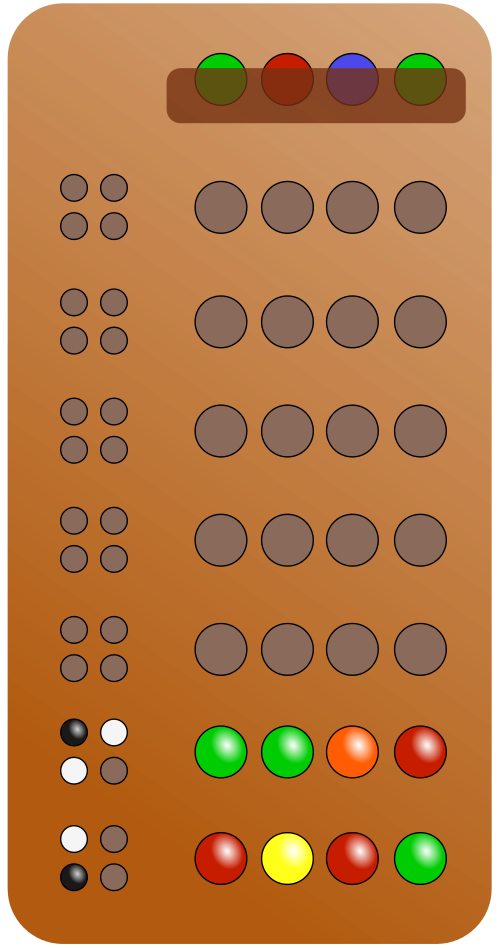
\includegraphics[width=0.25\textwidth]{pictures/mastermind.png}
  \vspace{-5mm}
  \end{center}
  \caption{Mastermind game (illustrative image)\protect\footnotemark.}
  \vspace{-5mm}
\end{wrapfigure}
\footnotetext{Image adopted from \url{http://commons.wikimedia.org/wiki/File:Mastermind\_beispiel.svg}, by Thomas Steiner under GFDL.}

The famous board game of \emph{Mastermind} is a prominent example.
The codemaker creates a puzzle for the codebreaker by choosing a
  combination of 4 coloured pegs (with colour repetitions allowed).
The codebreaker makes guesses, which are evaluated by the codemaker with
  black and white markers.
A black marker corresponds to a position at which the code and the guess matches.
A white marker means that some colour is present both in the code
  and in the guess but at different positions.

Another example is the \emph{counterfeit coin problem},
  the problem of identifying an odd-weight coin among
  authentic ones using just a balance scale.
The codemaker is not a real player here; the balance scale takes his function
  and evaluates the weighings performed by the codebreaker.
Numerous other examples can be found among various board games and logic puzzles,
 some of them being presented in the next chapter.

Code-breaking games bring many interesting problems to study.
Most importantly,
 \emph{how should the codebreaker play in order to minimize the number of experiments
   needed to undoubtedly determine the code?}
 \emph{Is there a strategy that would guarantee
   revealing the code in at most $k$ steps?}
 \emph{What strategy is optimal with respect
   to the average-case number of experiments,
   given that the code is selected
   from the given set with uniform distribution?}

Synthesis of an optimal strategy is a task computationally very intensive.
In some games, the optimal strategy might have a simple
  structure and can be described easily, such as in
  the counterfeit coin problem (see section \autoref{s:coins} for details).
In general, however, the strategy may have arbitrary structure and the only way
  to discover an optimal strategy is by considering all possible experiments
  in a given state and analysing the subproblems.

Therefore, one may prefer a suboptimal strategy or heuristics
  for experiment selection,
  which is easier to compute.
This brings another kind of problems.
Given a strategy,
  how can we compute the worst-case and the average-case number
  of experiments the strategy needs to reveal the code?

Mastermind and the counterfeit coin problem have been subjected to
heavy research and most of these questions are at least partially answered.
The exact results and summarization of the research in this area is presented
  in \autoref{ch:games}.
Nevertheless, few have been written about code-breaking games in general.
Some authors suggested general methods (and applied them on one of the games,
  e.g. \cite{cbg-stgopt, cbg-gen}),
  some vaguely stated that their approach can be applied
  to other games of the same kind but,
  to the best of our knowledge, no one has tried to
  create a general framework and provide
   results for code-breaking games in general.

Here comes this work to fill the gap.
We develop a general formalism that uses propositional logic to
  represent the secret code and the partial knowledge.
In short, the secret code is encoded as a valuation of
  a set of propositional variables
  and the codebreaker's goal is to discover the valuation
  using a series of experiments.
Each experiment can result in several outcomes,
  which are given in the form of a prepositional formula.

We study strategies for the games in general, with a focus on
  a special class of \emph{one-step look-ahead} strategies,
  strategy analysis and synthesis of an optimal strategy.
For these problems to be computationally feasible, one need to exploit
  symmetries of the game and neglect symmetric experiments during the analysis
  or strategy synthesis.
Algorithms for symmetry breaking in Mastermind
  based on graph isomorphism has been suggested in \cite{cbg-nauty}.
We generalize this approach and present
  an algorithm for elimination of symmetric experiments
  in general code-breaking games.

Main part of this thesis is a design of a computer language for
  code-breaking game specification
  and development of a computer program that
  loads a game from a file in the defined format
  and performs various tasks with the game.
We named the tool COBRA, the code-breaking game analyser.
Currently supported tasks are
\begin{itemize}
\item verify that a game specification is correct
  and sensible (overview mode),
\item simulate the game either interactively, with input from the user, or
  with decisions by specified strategies (simulation mode),
\item analyse a given strategy for experiment selection --
  compute the worst-case and average-case number of experiments needed (analysis mode),
\item synthesize the worst-case or average-case optimal strategy (optimal mode).
\end{itemize}
Using the tool, we can easily reproduce some of the known results
  for Mastermind and evaluate the same ideas in other code-breaking games.

The thesis is structured as follows.
Chapter 2 introduces several examples of code-breaking games,
  discusses known results, variants of the games and related research.
The general formalism, definitions and symmetry breaking approach
  are described in Chapter 3.
Chapter 4 is dedicated to our tool, COBRA, with description of its usage and
  abilities.
Experimental results with comparison of analysed strategies
  are presented in Chapter 5.
Finally, Chapter 6 concludes the work with many suggestions on future work
  and possible extensions of the tool.







\chapter[Examples of code-breaking games and existing results]{Game examples and existing results}
\label{ch:games}
We introduce a few examples of code-breaking games in this chapter.
The Counterfeit Coin problem and Mastermind game are quite well known,
  the other examples are based on various board games or less known
  logic puzzles.
We briefly summarize related research for each game, discuss
  its variations and applications and give a list of
  references.

Our goal in this work is neither to answer the research questions, nor
  to study possible generalizations.
We aim to create a general formalism and a computer language which could
  be used to describe arbitrary code-breaking game, if possible.
This chapter provides an overview of what we had in mind
  when we designed the framework and the language described
  in the rest of the thesis.

%%%%%%%%%%%%%%%%%%%%%%%%%%%%%%%%%%%%%%%%%%%%%%%%%%%%%%%%%%%%%%%%%%%%%%%%%%%%%%%%
\section{The counterfeit coin} \label{s:coins}

\begin{wrapfigure}{r}{0.26\textwidth}
  \begin{center}
  \vspace{-5mm}
  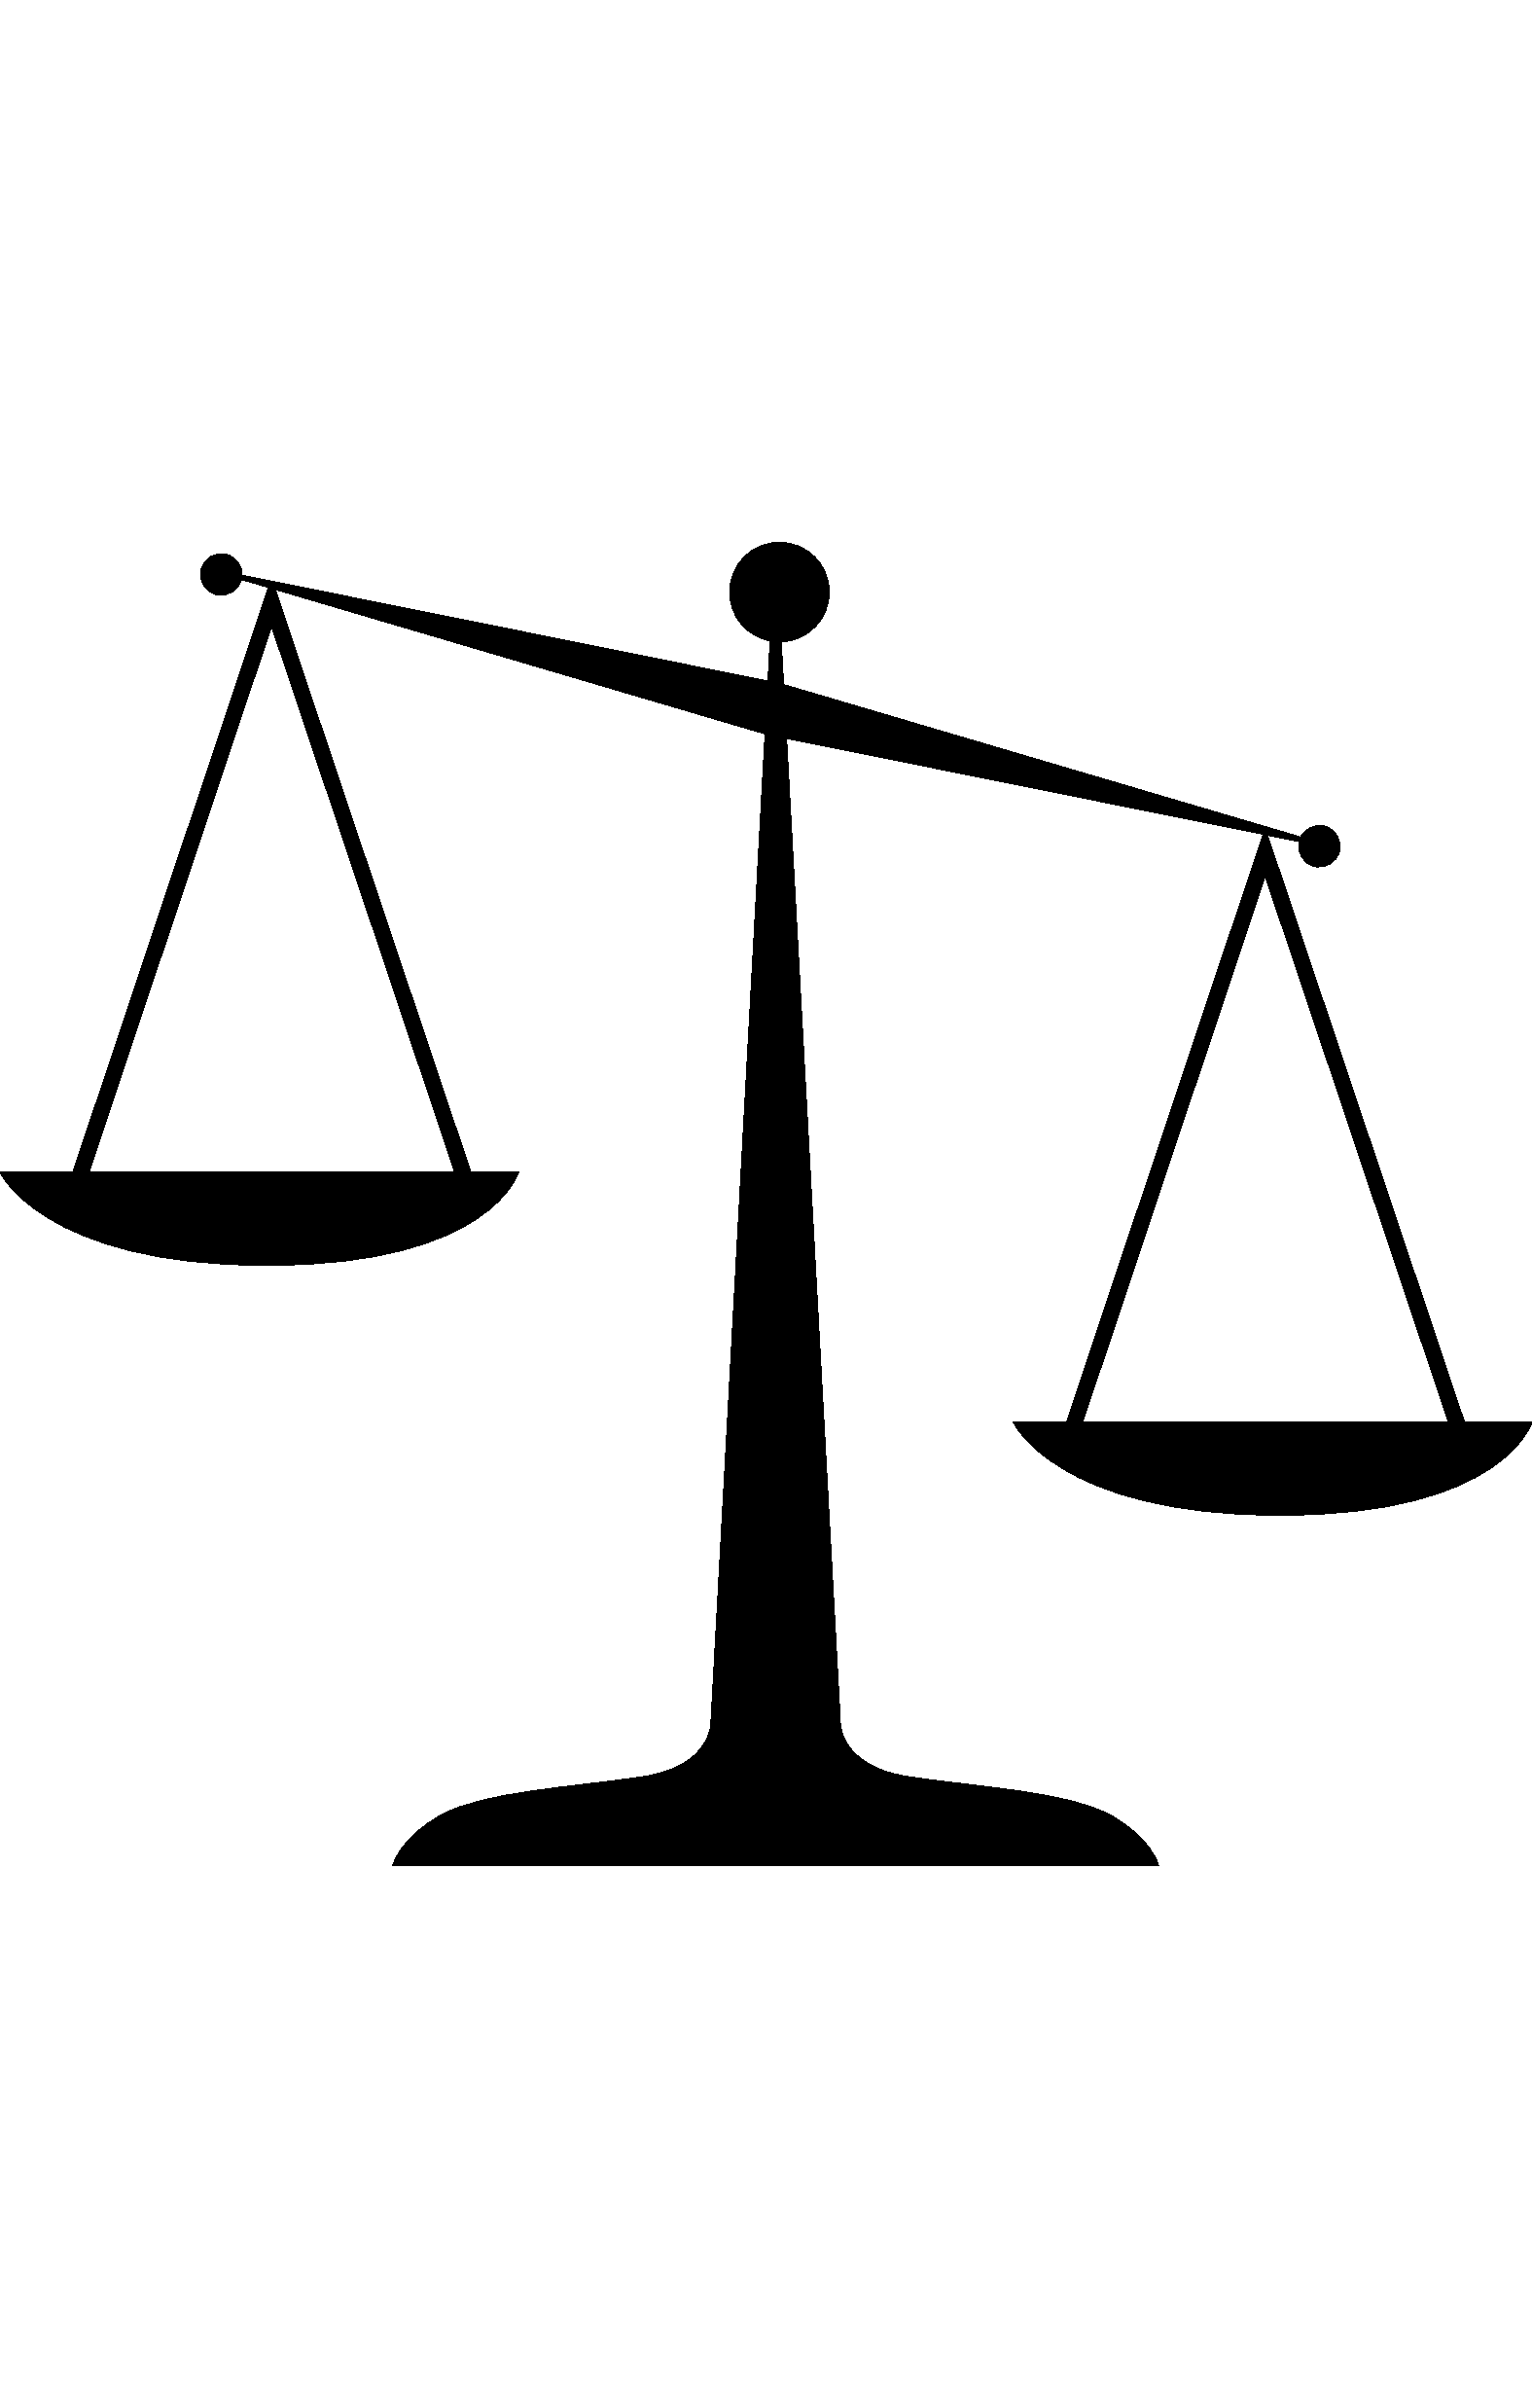
\includegraphics[width=0.23\textwidth]{pictures/scales.pdf}
  \vspace{-5mm}
  \end{center}
  \caption{Balance scale (illustrative image)\protect\footnotemark.}
  \vspace{-10mm}
\end{wrapfigure}
\footnotetext{Image adopted from
  \url{http://pixabay.com/en/justice-silhouette-scales-law-147214},
  under CC0 1.0 License.}

The problem of finding a counterfeit coin among regular coins in the fewest
  number of weighings on a balance scale is a folklore of
  recreational mathematics.

In all problems of this kind, you can only use the scale to weigh the coins.
You put some coins on the left pan, the same number of coins on the right pan
  and get one of the 3 possible outcomes.
Either both the sides weigh the same (denoted ``='')
  or the left side is lighter (``$<$''),
  or the right side is lighter (``$>$'').
The standard, easiest version can be formulated as follows.

\begin{problem}[The nine coin problem] \label{pr:coins9}
You are given $n >= 3$ (typically 9) coins, all except one having the same weight.
The counterfeit coin is known to be lighter.
Identify the counterfeit coin in minimal number of weighings.
\end{problem}

This problem is very easy as one can use \emph{ternary search} algorithm.
In short, we divide the coins into thirds, put one third against another
  on the scale.
If both pans weigh the same, the counterfeit coin must be in the last third,
  otherwise it must be on the lighter pan.
In this way, the size of the search space is reduced
  by a factor of 3 in each step, which is optimal.

In 1940s, more complicated version was introduced by Grossman\cite{coins-grossman1945}.

%whether the counterfeit coin is underweight or overweight
\begin{problem}[The twelve coin problem] \label{pr:coins12}
You are given $n >= 3$ (typically 12) coins, all except one having the same weight.
It is not known whether the counterfeit coin is heavier or lighter.
Identify the counterfeit coin and its weight relative to others
  in minimal number of weighings.
\end{problem}

The optimal solution for $n=12$ requires 3 weighings.
One of the optimal
  strategies is shown in \autoref{fig:coins12tree} as a decision tree.

\begin{figure}[h]
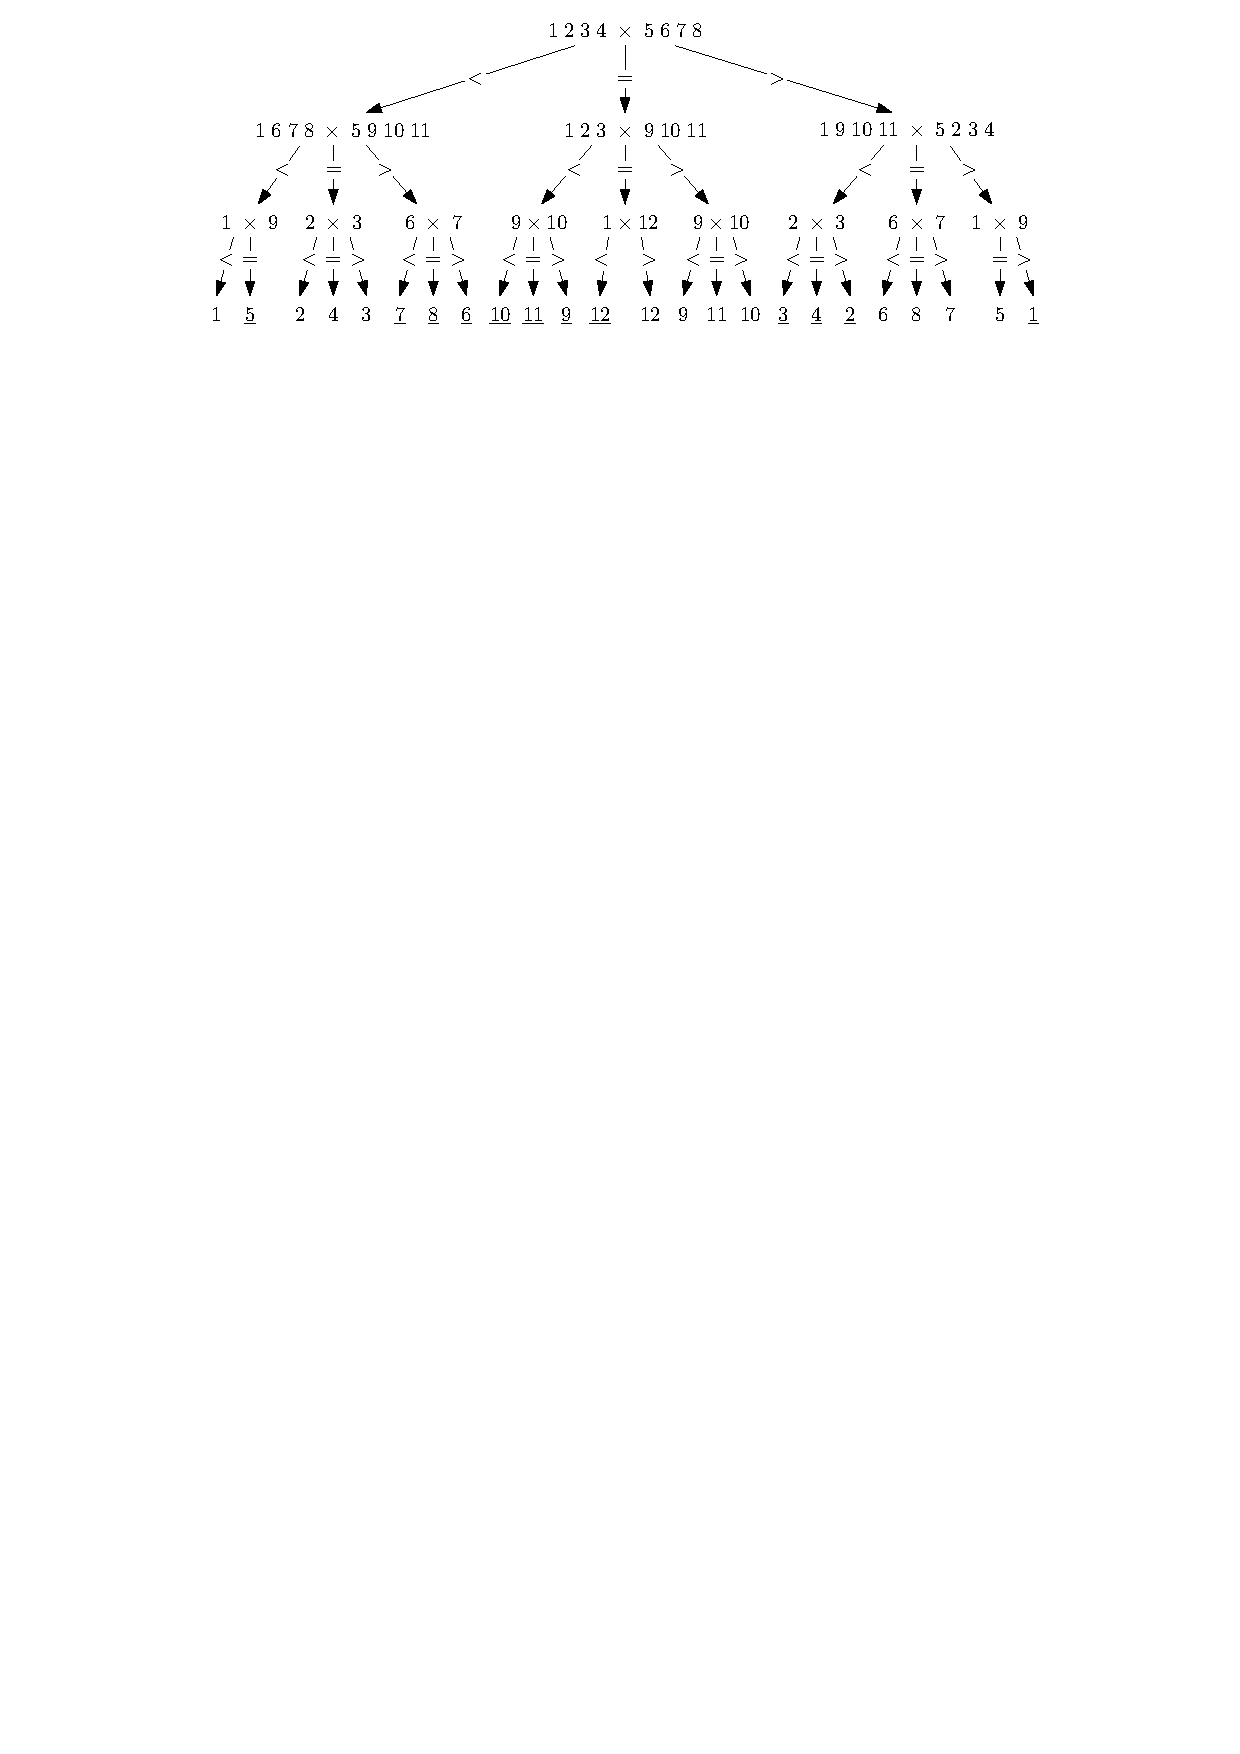
\includegraphics[width=\textwidth]{pictures/coins12.pdf}
\caption{Decision tree for The Twelve Coin Problem. \\
Leaf $x$ means that the coin number $x$ is lighter, $\underline{x}$ means that
the coin number $x$ is heavier.}
\label{fig:coins12tree}
\end{figure}

\subsection{Known results}

The research usually focuses on bounds on the maximal value of $n$
  for which the problem can be solved in $w$ weighings, for a given $w$.
Thus a solution of a problem is usually formulated as a theorem like the
  following one.

\begin{theorem}[Dyson, \cite{coins-dyson1946}]\label{th:coins12}
There exists a strategy that identifies the counterfeit coin and
  its type as described in \autoref{pr:coins12} with $w$ weighings,
  if and only if
  \[ 3 <= n <=\frac{3^w - 3}{2}. \]
\end{theorem}

\begin{proof}
We show the main part of the original Dyson's proof\cite{coins-dyson1946}
  here because of its elegant combinatorial idea.
We show a scheme for $n = \frac{1}{2}(3^w - 3)$.

Let us number the coins from $1$ to $n$.
To a coin number $i$, we assign
  two labels from $\{0,1,2\}^w$ -- those corresponding to the numbers
  $i$ and $3^w - 1 - i$ in ternary form.
Notice that all possible labels are used exactly once, except for $0^w, 1^w$
  and $2^w$, which were not assigned to any coin.
The labelling has the property that you can
  get one label of a coin from another by substituting $0$ by $2$ and $2$ by $0$.

A label is called ``clockwise'' if the first change of digit in it is
the change from $0$ to $1$, from $1$ to $2$, or from $2$ to $0$.
Otherwise, it is called ``anticlockwise''.
Thanks to the property we mentioned, one of the labels of a coin is always
  clockwise and the other is anticlockwise.

Let $C(i, d)$ be a set of coins such that $i$-th symbol in
  its clockwise label is $d$.
Since a permutation changing $0$ to $1$, $1$ to $2$ and $2$ to $0$ transfers
  coins from $C(i,0)$ to $C(i,1)$,
        from $C(i,1)$ to $C(i,2)$ and
        from $C(i,2)$ to $C(i,0)$,
  all the sets $C(i, d)$ contain exactly $n/3$ coins.
Now, let $i$-th experiment be the weighing of the coins $C(i,0)$ against $C(i, 2)$.
It remains to show that the experiments uniquely determine the counterfeit coin.
Let $a_i$ be 0, 1, or 2 if the result of $i$-th experiment is
  left side is lighter, both are the same, or right side is lighter, respectively.

If the counterfeit code is overweight, the $i$-th symbol of its clockwise label
  must be $a_i$. On the other hand, if it is underweight, the $i$-th symbol of
  its anticlockwise label must be $a_i$.
The solution of the problem is therefore the coin with the label $a_1a_2...a_w$
  and is heavier than others if and only if this label is clockwise.
\autoref{fig:coins12scheme} shows an example of the construction for
  $n = 12 = \frac{1}{2}(3^3 - 3)$, clockwise labels printed in bold.

\begin{figure}[h]
\begin{center}
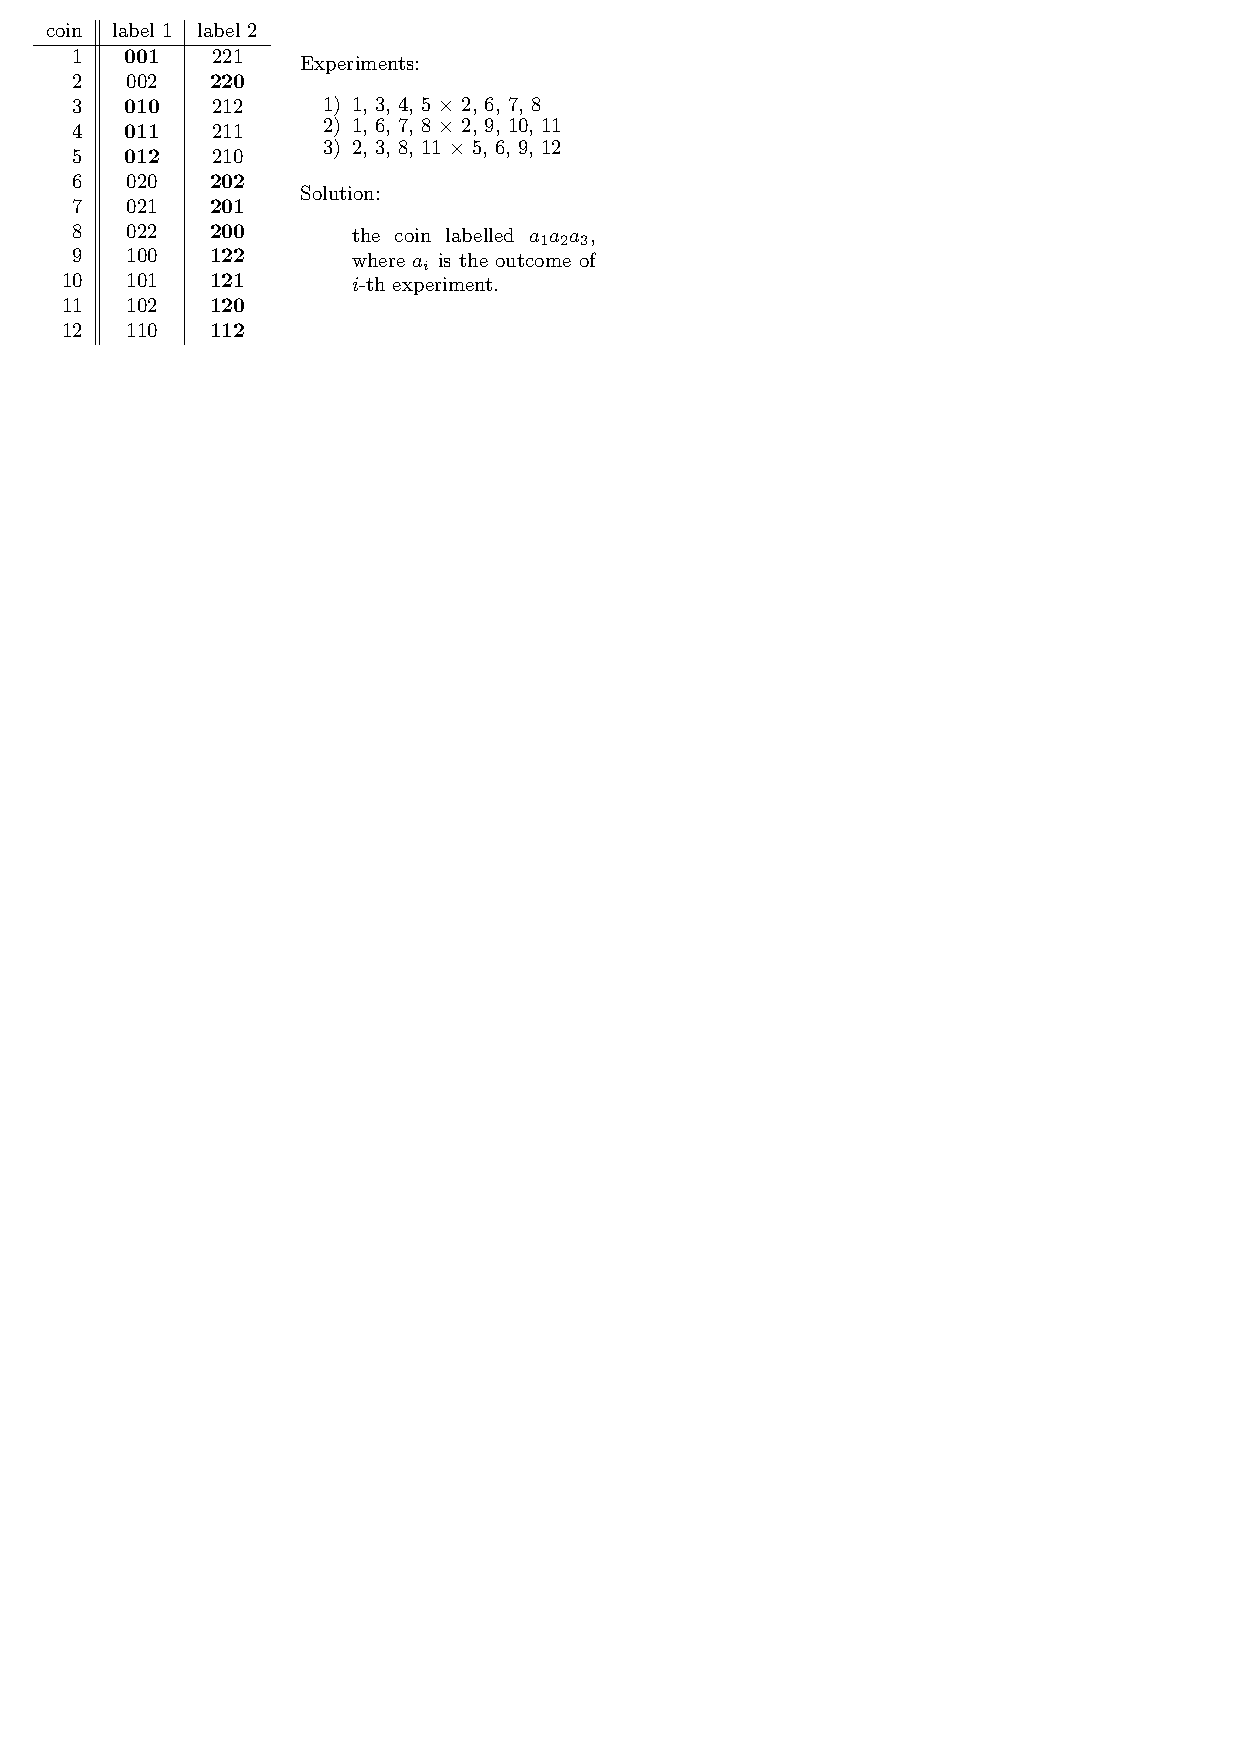
\includegraphics{pictures/coins12-th.pdf}
\end{center}
\caption{Demonstration of the ternary label construction for $n=12$.}
\label{fig:coins12scheme}
\end{figure}

The case $n < \frac{1}{2}(3^w - 3)$ can be solved similarly with some modifications
  to the labelling.
However, the scheme makes use of a genuine coin that was discovered in the first
  weighing and, therefore, the following experiments depend on the outcome of
  the first.
Finally, the proof that the coin cannot be identified for
  $n > \frac{1}{2}(3^w - 3)$ can be carried out using information theory.\qed
\end{proof}

\subsection{Generalizations and related research}

Naturally, the problem has been generalized in various ways and
  studied by many authors.
In ``Coin-Weighing Problems''\cite{coins-cwproblems1995}, Guy and Nowakovski
  gave a great overview of the research in the area until 1990s
  with an extensive list of references.
We list the most interesting variations and generalizations below.

\begin{description}
\item[Weight of counterfeit coin.]
  Either it is known whether the counterfeit coin is lighter or heavier,
  or it is not.
  The first one allows for more generalizations due to its simpler nature
  but both problems have been heavily researched.
\item[Number of counterfeit coins.]
  In the most common case, there is exactly one counterfeit coin,
    which allows for natural generalizations.
  First, a variation of \autoref{pr:coins9} with 2 or 3 counterfeit coins
   was studied\cite{coins-2fakes}\cite{coins-3fakes},
  then with $m$ counterfeit coins in general\cite{coins-mfakes}.
  Some authors studied the problem for unknown number of
  counterfeit coins\cite{coins-unknownfakes},
  or for \emph{at most} $m$ counterfeit coins\cite{coins-atmostfakes}.
\item[Additional regular coin(s).]
  In some cases, it may help if you are given an additional coin (or more coins),
    which is guaranteed not to be counterfeit.
  For example, for $n = 13$ in \autoref{pr:coins12}, you need 4 weighings.
  However, if you are given this one extra coin, you can determine the
    solution in just 3 weighings\cite{coins-dyson1946}.
\item[Non-adaptive strategies.]
  In this popular variation of the problem you have to announce all experiments
    in advance and then just collect the result.
  In other words, later weighings must not depend on the outcomes of the earlier weighings.
  Notice that the scheme constructed in the proof of \autoref{th:coins12} for
  $n = \frac{1}{2}(3^w - w)$ is indeed non-adaptive.
  However, the original proof uses an adaptive scheme for a smaller $n$.
  This was later updated, showing that there always exists an optimal scheme for
  \autoref{pr:coins12} which is non-adaptive\cite{coins-nonadaptive}.
\item[Unreliable balance.]
  This generalization introduces the possibility that
  one (or more) answers may be erroneous.
  The problem of errors/lies in general deductive games is well studied,
    see \cite{games-lies}.
  It was applied on the counterfeit coin problem (\autoref{pr:coins9} variant)
  in \cite{coins-unreliable} with at most one erroneous outcome or in
  \cite{coins-unreliable2} with two.
\item[Multi-pan balance scale.]
  In this variation, your balance scale has $k$ pans.
  You put the same number of coins on every pan and
    you get either the information that all
    weigh the same or which arm is lighter or heavier
    than others\cite{coins-multiplearm}.
\item[Parallel weighing.]
  In this generalization, you have 2 (or $k$, in general)
    balance scales, you can weigh different coins on
    the two scales simultaneously and it counts
    as one experiment only\cite{coins-parallel}.
  The motivation here is that weighing takes significant time,
  you have more scales and strive to minimize the time the whole process takes.
\end{description}

%%%%%%%%%%%%%%%%%%%%%%%%%%%%%%%%%%%%%%%%%%%%%%%%%%%%%%%%%%%%%%%%%%%%%%%%%%%%%%%%
\section{Mastermind} \label{sec:mm}

\emph{Mastermind} is a classic code-breaking board game for 2 players,
  invented by Mordecai Meirowitz in 1970.
One player has the role of a \emph{codemaker} and the other of a \emph{codebreaker}.
First, the codemaker chooses a secret code of $n$ coloured pegs.
Then a codebreaker tries to reveal the code by making guesses.
The codemaker evaluates the guesses using black and white markers.
Black markers correspond to positions at which the code and the guess matches,
  a white marker means that some colour appears both in the code and in the guess,
  but at different positions.
The markers in the answer are not ordered, so the codebreaker does not know,
  which marker correspond to which peg in the guess.
Codebreaker's aim is to find out the code in minimal number of guesses.

More formally, let $C$ be a set of colours of size $c$.
Define a distance $d : C^n\times C^n -> \Nseto\times\Nseto$
  of two colour sequences by $d(u, v) = (b, w)$, where
\[
b = |\{ i \in\Nset \| u[i] = v[i] \}|
\]
\[
w = \sum_{j\in C} \min\big(\big|\{ i \| u[i] = j \}\big|,\;
                           \big|\{ i \| v[i] = j\}\big|\big)  - b.
\]
If the codemaker's secret code is $h$ and the codebreaker's guess is $g$,
  the guess should be evaluated with $b$ black pegs and $w$ white pegs, where
  $(b,w) = d(h,g)$.
Therefore, if the codebreaker have guessed $g_1, g_2, ..., g_k$ and the results
  were $(b_1,w_1), ..., (b_k, w_k)$,
  the search space is reduced to codes
  \[
  \{ u\in C^n \| \forall i<=k.\; d(u, g_i) = (b_i,w_i)\}.
  \]

\begin{wrapfigure}{r}{0.32\textwidth}
  \vspace{-5mm}
  \begin{center}
  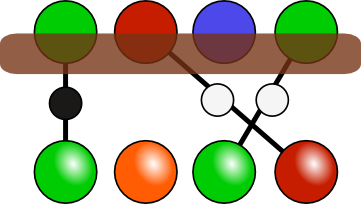
\includegraphics[width=0.25\textwidth]{pictures/mastermind-matching.png}
  \end{center}
  \caption{Guess evaluation by maximal matching.}
  \vspace{-5mm}
\end{wrapfigure}

\newcommand{\incode}[1]{#1^\bullet}
\newcommand{\inguess}[1]{#1_\bullet}

Another way of looking at the guess evaluation is using
  \emph{maximal matching} of the pegs in the code $h$ and the guess $g$.
A matching is a set of pair-wise non-adjacent edges between
  the pegs in the guess (represented by $\inguess{i}$ for $1<=i<=n$) and
  the pegs in the code (represented by $\incode{i}$ for $1<=i<=n$).
Let $M$ be a maximal matching such that

\begin{enumerate}
\item an edge connects only pegs of the same colour, i.e. if $(\inguess{i},\incode{j})\in M$, then $h[i] = g[j]$, and
\item if $h[i] = g[i]$ then $(\inguess{i},\incode{i})\in M$.
\end{enumerate}

Maximal means that no edge can be added without breaking one of the conditions.
The edges in $M$ correspond to the markers in the response,
  a marker being black if and only if the corresponding edge connects $\inguess{i}$
  with $\incode{i}$ for some $i$.

\subsection{Known results and related research}

Much research has been done on this game, authors focusing
  on \emph{exact values}, \emph{asymptotics} (e.g. \cite{mm-chvatal}), or
  computer generated strategies.
One of the fundamental theoretical results is that
  \emph{Mastermind satisfiability problem}, asking
  whether there exists at least one valid solution,
  given a set of guesses and their scores, is NP-complete\cite{mm-np}.

When focusing on strategy synthesis, the goal is either to minimize
  \emph{the maximal number of guesses}
  or \emph{the expected number of guesses}, given that the code
  is selected from the set of possible codes with uniform distribution.
These two problems are quite different and strategies performing well
  in one case may perform poorly in the other.

Knuth\cite{mm-knuth} proposes a strategy that chooses a guess
  that minimizes the maximal number of remaining possibilities over all
  possible responses by the codemaker.
This strategy requires at most 5 guesses in the standard $n=4$, $c=6$ variant,
  which can be shown optimal.
In the average case, the strategy makes $4.48$ guesses.

Other authors proposed other \emph{one-step look-ahead} strategies.
Irving\cite{mm-expnum} suggested minimizing the expected number
  of remaining possibilities,
Neuwirth\cite{mm-entropy} maximized the entropy of the number
  of possibilities in the next round.
Much later, Kooi\cite{mm-mostparts} came up with a simple strategy that
  maximizes the number of possible responses by the codemaker,
  which is computationally easier and performs better that the previous two.

Using a backtracking algorithm, Koyama and Lai\cite{mm-exp-opt} found
  the optimal strategy for the expected case, which requires $4.34$
  guesses on average.
The comparison of the described strategies is shown in \autoref{tbl:one-step}.

\begin{table}[h]
\begin{center}
\begin{tabular}{|l|c|c|c|}
\hline Strategy & First guess & Expected-case & Worst-case \\ \hline
Maximal num. & AABB & 4.476 & 5 \\ \hline
Expected num. & AABC & 4.395/4.602\footnotemark & 6 \\ \hline
Entropy & ABCD & 4.416 & 6 \\ \hline
Most parts & AABC & 4.373 & 6 \\ \hline
Exp-case optimal & AABC & 4.340 & 6 \\ \hline
\end{tabular}
\caption{Comparison of one-step look-ahead strategies. Data from \cite{mm-ville} and \cite{mm-mostparts}.}
\label{tbl:one-step}
\end{center}
\end{table}
\footnotetext{Irwing's paper reports 4.395 as the expected number
 of experiments of this strategy.
 However, he states that his strategy selects the first two experiments
 on the basis of the expected number of models and the rest is done by
 exhaustive search.
 We were not able to reproduce this result and the
 paper contains several other irreproducible results,
 which has been already pointed out in \cite{mm-mostparts}.
 The number reported by our tool when using this strategy only is 4.602.}

Apart from \emph{one-step look-ahead} strategies, which are, in general,
  computationally intensive and do not scale well for bigger $n$ or $c$,
  other approaches has been suggested.
Many authors tried to apply genetic algorithms
  (see \cite{mm-ga} for an exhaustive overview and references therein),
  other analysed various heuristic methods (e.g. \cite{mm-heuristic}).

\subsection{Variations and applications}

\begin{description}
\item[Bulls and Cows]
is an old game with a principle very similar to Mastermind.
The only difference is that it uses digits instead of colours and does not allow repetitions.
Slovesnov wrote an exhaustive analysis of the problem, see \cite{bullsandcows}.


\item[Static Mastermind] is a variation of the game in which all guesses
  must be made in one go.
The codebreaker prepares a set of guesses,
  then the codemakers evaluates all of them as usual and
  the codebreaker must determine the code from the outcomes.
This variation was introduced by Chvátal\cite{mm-chvatal} and
  partially solved (for $n<=4$) by Goddard\cite{mm-static},
  proving that for $4$ pegs and $k$ colours,
  the optimal strategy uses $k-1$ guesses.
Note that this corresponds to so-called \emph{non-adaptive} strategies
  for the Counterfeit Coin problem.

\item[String matching,] also called
  \emph{Mastermind with black-markers only}
  is a variation without white markers, i.e.
  you make guesses and the only information you get is the
  number of positions at which your guess is correct.
This problem was already studied by Erdős\cite{erdos-two}, who gave some
  asymptotic results about the worst-case number of guesses.
Later, this problem found an application in genetics with a need of
  methods to select a subset of genotyped individuals for phenotyping
  \cite{mm-app-gen2}\cite{mm-app-gen}.

\item[Extended Mastermind] was introduced by Focardi and Luccio,
  who showed that it is strictly related to cracking bank PINs for accessing ATMs
  by so-called \emph{decimalization attacks}\cite{mm-pins}.
In this variation, a guess is not just a sequence of colours, but a sequence of
  sets of colours. For example, if we have six colours $\{A, B, C, D, E, F\}$
  and the code is $AECA$,
  you can make a guess $\{A\}, \{C,D,E\}, \{A,B\}, \{F\}$, which
  will be awarded two black markers (for the first two positions)
  and one white marker (for $A$ guessed at position 3).
\end{description}

%%%%%%%%%%%%%%%%%%%%%%%%%%%%%%%%%%%%%%%%%%%%%%%%%%%%%%%%%%%%%%%%%%%%%%%%%%%%%%%%
\section{Other games}
\subsection{Black Box}

Black Box is a code-breaking board game in which one player creates a
  puzzle by placing four marbles on a $8\times 8$ grid.
The other player's goal is to discover their positions
  by the use of ``rays''.
The codebreaker chooses a side of the grid and an exact row/column, in which
  the ray enters the grid (thus having 32 choices).
For each ray, the codemaker announces the position, where the ray emerged from the grid,
  or says ``hit'', if the ray directly hit a marble\cite{blackbox}.

The marbles interact with rays in three ways:
\begin{description}
\item[Hit.] If a ray fired into the grid directly strikes a marble,
  the result is ``hit'' and the ray does not emerge from the box.
\item[Deflection.] If a ray does not directly strike a marble,
  but it should pass to one side of a marble, the ray is
  ``deflected'' and changes its direction by 90 degrees.
\item[Reflection.] If a ray should enter a cell with marbles on both sides,
  than it is ``reflected'' and returns back the same way it came.
  The same happens if a marble is at the edge of the grid
  and a ray is fired from a position next to it (so that it should be deflected
  even before entering the box according to the second rule).
\end{description}

\begin{figure}[h]
\begin{center}
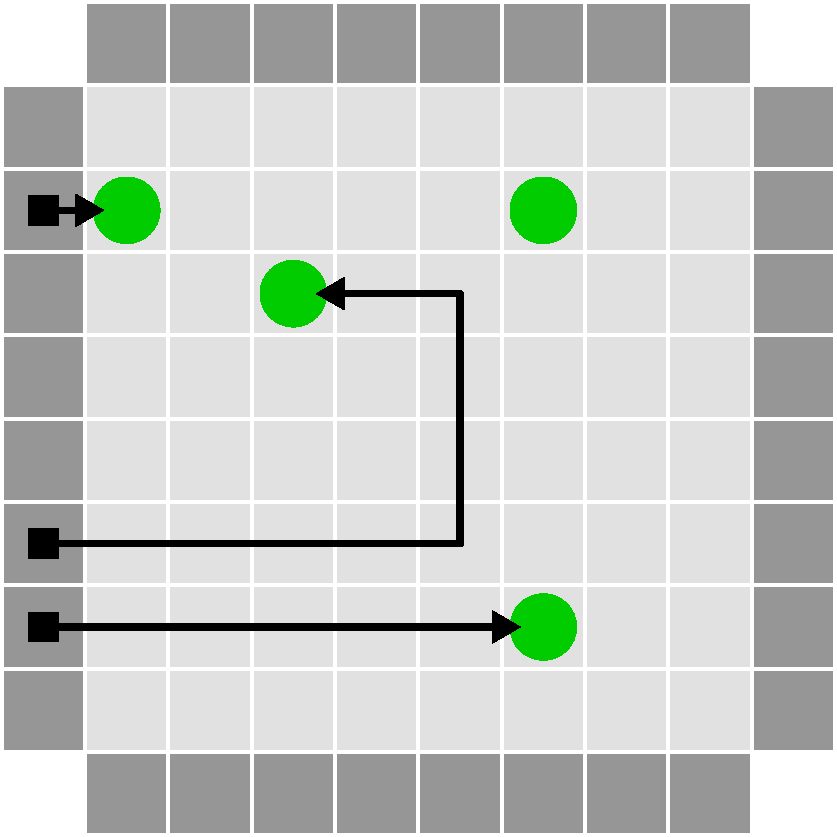
\includegraphics[width=.3\textwidth]{pictures/blackbox2.pdf} ~
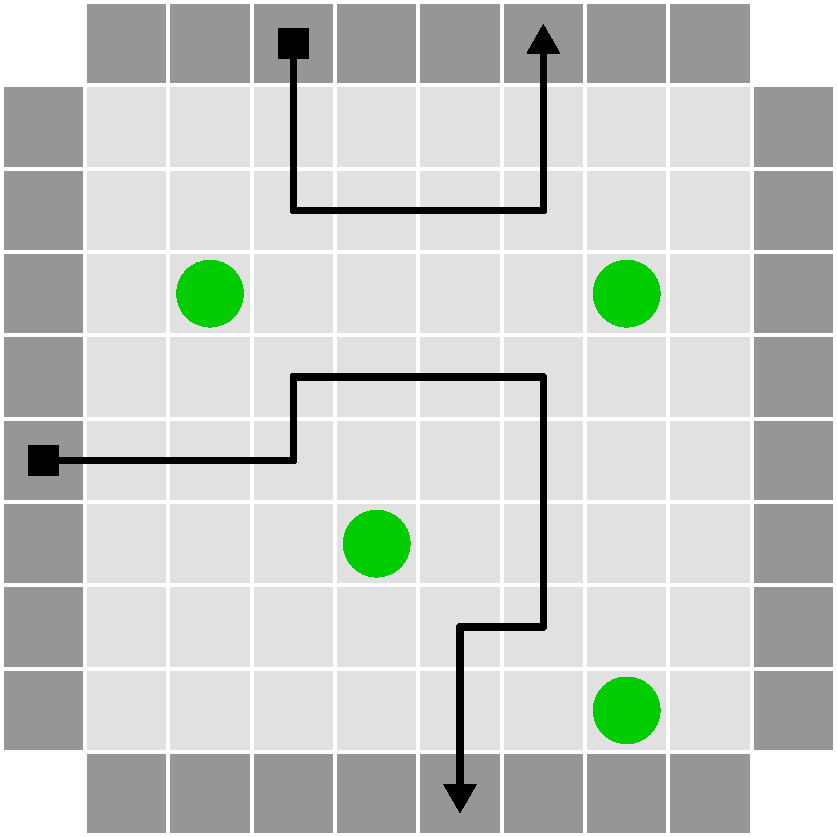
\includegraphics[width=.3\textwidth]{pictures/blackbox1.pdf} ~
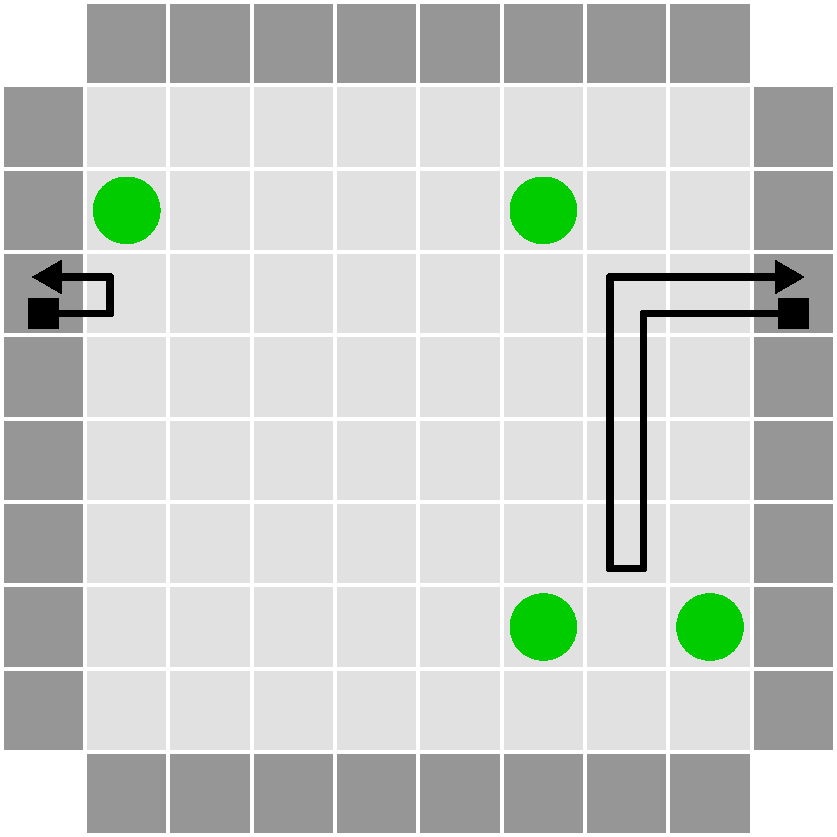
\includegraphics[width=.3\textwidth]{pictures/blackbox3.pdf} ~
\end{center}
\caption{Illustration of the rules of Black Box game\protect\footnotemark.}
\label{fig:blackbox-rules}
\end{figure}

\addtocounter{footnote}{-1}
\begin{wrapfigure}{r}{0.35\textwidth}
  \vspace{-10mm}
  \begin{center}
  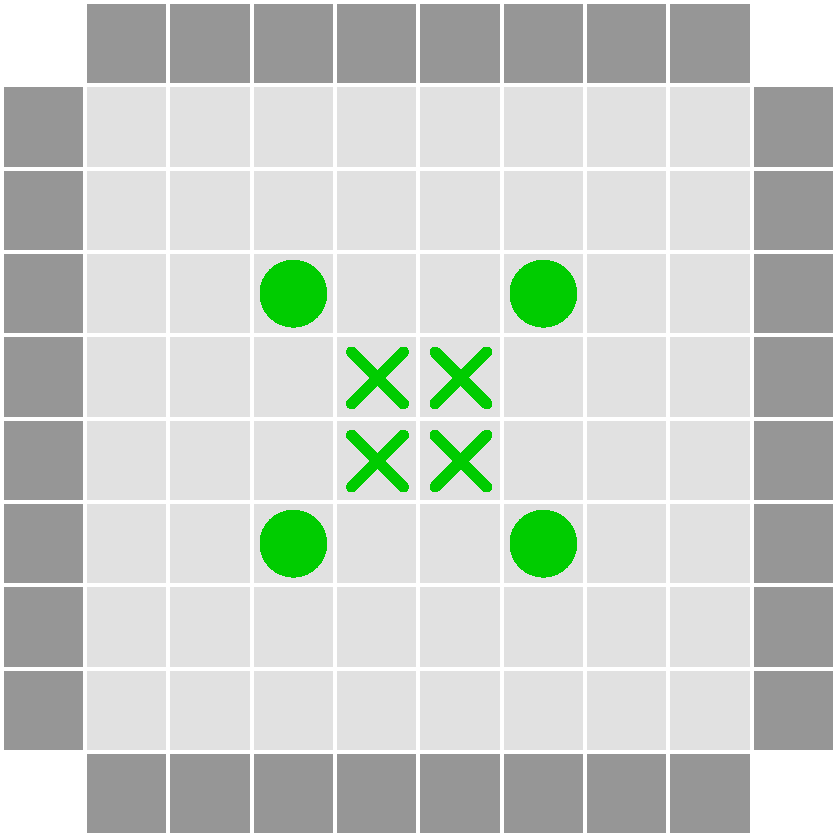
\includegraphics[width=0.3\textwidth]{pictures/blackbox-a.pdf}
  \end{center}
  \caption{An example of ambigous configuration\protect\footnotemark.}
  \label{fig:blackbox-ambigous}
\end{wrapfigure}

\footnotetext{Images adopted from \url{http://en.wikipedia.org/wiki/Black\_Box\_(game)} under GFDL 1.2. with minor modifications.}

A few examples are shown in \autoref{fig:blackbox-rules}.
The first image shows cases in which the ray hits the marble,
  the second shows rays deflected multiple times, emerging from
  the box at a different place, and the third demonstrates
  the two cases in which reflection happens.

Note that if the game is played with 5 or more marbles,
  they can be placed in the grid so that their position can
  not be uniquely determined.
\autoref{fig:blackbox-ambigous} shows an example of such
  problematic configuration.

Although Black Box is an interesting example of a code breaking game,
  there are configurations for which the codebreaker has to fire a ray from
  all positions to discover the marbles
  (and, for $5$ or more marbles, it may even be impossible),
  which makes the game uninteresting from a research point of view.

However, the game has become a popular puzzle for children and
  its principle has been used in other board games such as \emph{Laser maze}\cite{lasermaze}.

\subsection{Code 777}

During the board game named \emph{Code 777}, players sit in a circle,
  each drawing three cards at the beginning.
Players must not look at their own cards but they put them to a rack in front of them
  so that other players can see them.
Each card has one of seven colours and contains a number from one to seven.
The goal of the game is to determine which cards you have, using questions like
 ``Do you see more yellow sevens or blue fives?'', which the others answer\cite{code777}.

We can reformulate this as a code-breaking game, in which a player
  receives some cards, each having several attributes, each of which can have
  multiple values.
A player's goal is to determine his cards using questions
  like ``Do I have more [A] or [B]'', where [A] and [B] are conditions on
  any subset of attributes.
For example, if the attributes are number, colour, and shape, one can ask
  ``Do I have more triangles or green twos?''.

\subsection{Bags of gold}

Imagine you have 10 bags of gold coins and
  you know that all coins in one bag are the same.
You were tipped off that some of the bags may contain counterfeit coins,
  which weigh 9 grams instead of 10 but are indistinguishable otherwise.
Suppose all coins in one bag are the same.
You have a digital scale that can show you exact weight of a set of coins.
How to find out which bags contain counterfeit coin in
  the minimal number of weighings?
Suppose there is a sufficient number of coins in each bag.

In the original version of this riddle, the scale has unlimited capacity and
  there is only one bag of counterfeit coins.
In that case, the secret can be determined in a single experiment.
You take one coin from the first bag, two coins from the second and so on up to
  10 coins from the last.
You put all those 55 coins on the scale and, if they are all good,
  they weigh 550 grams.
If the weight is by $x$ grams lower, you know that there are $x$ counterfeit
  coins in your set and, therefore,
  the $x$-th bag is the one with counterfeit coins.

The game gets more interesting if the capacity of the scale is limited, or
  if we have more bags and the number of coins in them is limited.
A special case, in which each bag contains a single coin is
  studied in \cite{erdos-two}, and is shown to be similar to the
  string matching problem (Mastermind with black-markers only).
Otherwise, the game lives only in a form of a logic puzzle and,
  to the best of our knowledge, no general results have been found.

\chapter{Code-breaking Games}

% znaceni
\newcommand{\Val}{V} % mnoz vsech valuaci
\newcommand{\val}{v} % jedna valuace
\newcommand{\numval}{\tau} % number of sat valutaions
\renewcommand{\Form}{\textrm{Form}} % mnoz vsech formuli
\newcommand{\form}{\varphi} % jedna formule
\newcommand{\aform}[1]{\form_{0..#1}} % accumulated formula

% code-breaking game
\newcommand{\game}{\mathcal{G}}
\newcommand{\Var}{X}
\newcommand{\init}{\varphi_0}
\newcommand{\Expt}{T}
\newcommand{\expt}{t}
\newcommand{\Exp}{E}
\renewcommand{\exp}{e}
%\newcommand{\Param}{\Pi}
\newcommand{\param}{p}
\newcommand{\infer}{\Phi}

% dalsi veci
\newcommand{\Perm}{\textrm{Perm}}
\newcommand{\perm}{\pi}
\newcommand{\result}{\rho}

% nep
\newcommand{\stg}{\sigma}

\newcommand{\proc}{\pi}
\newcommand{\procstg}[2]{\proc_{#1,#2}}

\newcommand{\len}{\lambda}
\newcommand{\lenstg}[2]{\len^{#1,#2}}
\newcommand{\lenmax}[1]{\len^{#1}}
\newcommand{\lenexp}[1]{\len^{#1}_\textrm{exp}}

\newcommand{\exactly}[1]{\textrm{Exactly-#1}\:}
\newcommand{\atleast}[1]{\textrm{AtLeast-#1}\:}
\newcommand{\atmost}[1]{\textrm{AtMost-#1}\:}

\section[0]{Notation}
Let $\Form_\Var$ be the set of all formulas over the set of prepositional variables $\Var$;
$\Val_\Var$ be the set of all valuations of variables $\Var$.
Formulas $\form_0, \form_1 \in \Form_\Var$ are (semantically) equivalent,
  written $\form_0 \equiv \form_1$, if
  $\val(\form_0) = \val(\form_1)$ for all $\val\in\Val_\Var$.
For a formula $\form\in\Form_\Var$, let
  $\numval_\Var(\form) = |\{ \val\in\Val_\Var \| \val(\form) = 1 \}|$
  be the number of valuations by which $\form$ is satisfied.
We often omit the index $\Var$ if it is clear from the context.

For any unary predicate $P$, $\#i\in A.P(i) = |\{ i\in A \| P(i)\}|$.
  We often omit the ``$\in A$'' part and write only $\#i.P(i)$
  if the range of $i$ is clear from the context.

Let $\Perm_\Var$ be the set of all permutations of $\Var$.

%-------------------------------------------------------------------------------
% DEF: CODE BREAKING GAME
\section{Formal definition}
\begin{definition} \label{def-game}
A \emph{code-breaking game} is a quintuple
  $\game = (\Var, \init, \Expt, \Exp, \infer)$, where
  \begin{itemize}
  \item $\Var$ is a finite set of propositional variables,
  \item $\init \in \Form_\Var$ is a satisfiable prepositional formula,
  \item $\Expt$ is a finite set of types of experiments,
  \item $\Exp \subseteq \Expt \times \Var^\star$ is an \emph{experiment} relation,
  and
  \item $\infer: \Val_\Var \times \Exp -> \Form_\Var$ is an
  \emph{inference function} such that
    \begin{enumerate}[label=(\roman*)]
    \item $\forall\val\in\Val_\Var, \exp\in\Exp$:
      $\val(\infer(\val, \exp)) = 1$ and
    \item $\forall\val\in\Val_\Var, (\expt, \param)\in\Exp, \perm\in \Perm_\Var$:
        \[
        \init \equiv \perm(\init) \;==>\;
          \infer(\val, (\expt, \perm(\param)))
          \equiv
          \perm(\infer(\val, (\expt, \param))).
        \]
    \end{enumerate}
 \end{itemize}
\end{definition}

Intuitively, the objective of the game is to find a valuation of
  variables $\Var$ by a series of experiments.
Let us call it \emph{the wanted valuation}.
The search space is reduced by formula $\init$,
  which is always known to be satisfied by the wanted valuation.

Experiments consist of a type, which is from the set $\Expt$ and a
  parametrization, which is a string of variables from $\Var$.
The experiment relation $\Exp$ specifies all permitted parametrizations
  for each type of experiment and, therefore, $\Exp$ is the set of
  all possible experiments as pairs.

The inference function is the entity that evaluates the experiment.
Given the wanted valuation and an experiment, it gives the player
  partial information about the valuation,
  in the form of a formula that is guaranteed
  to be satisfied by the wanted valuation (see condition (i)).
Put simply, condition (ii) says that if $\perm$ is a symmetry
  of the initial formula $\init$, we do not get different information
  if we permutate the variables in the parametrization of the experiment
  by $\perm$.

%-------------------------------------------------------------------------------
% EXAMPLE: FAKE-COIN PROBLEM

\begin{example}[Fake-coin problem]
Fake-coin problem with $n$ coins, one of which is fake, can be formalized as
a code breaking game
$\mathcal{F}_n = (\Var, \init, \Expt, \Exp, \infer)$, where

\begin{itemize}
\item
$\Var = \{x_1, x_2, ..., x_n, y\}$ \\
Intuitively, variable $x_i$ tells weather the coin $i$ is fake.
Variable $y$ tells weather it's lighter or heavier.

\item
$\init = \exactly{1}(\{x_1, ..., x_n\})$ \\
This is to ensure that exactly one coin is fake.

\item
$\Expt = \{\expt\}$ \\
There is only one type of experiment -- weighting the coins.

\item
$\Exp = \{ (\expt, \param) \|
  \param \in \{x_1, ..., x_n\}^{2n},
  n >= 0,
  \forall x\in\Var: \#_x(\param)<=1 \} $\\
Any sequence of variables of even length with no repetitions
  is a permitted parametrization of type $\expt$.

\item
$\infer(\val, (\expt, \param)) = \left\{
\begin{array}{ll}
(\bigvee A \wedge \neg y) \vee (\bigvee B \wedge y) &
    \textrm{if r = lighter,} \\
(\bigvee A \wedge y) \vee (\bigvee B \wedge \neg y) &
    \textrm{if r = heavier,} \\
\neg \bigvee(A\cup B) &
    \textrm{if r = equal,}
\end{array} \right.$

where
$A = \{ \param[i] \| 1 <= i <= |\param|/2 \}$,
$B = \{ \param[i] \| |\param|/2 < i <= |\param| \}$.
The conditions correspond to the result $r$ of the experiment:
\begin{itemize}
\item r = lighter if $(v(c) = 1$ for some $c\in A$ and $v(y) = 0)$
  or $(v(c) = 1$ for some $c \in B$ and $v(y) = 1)$
\item r = heavier if $(v(c) = 1$ for some $c\in A$ and $v(y) = 1)$
  or $(v(c) = 1$ for some $c \in B$ and $v(y) = 0)$
\item r = equal if $v(c) = 0$ for every $c\in A\cup B$
\end{itemize}
\end{itemize}
\end{example}

%-------------------------------------------------------------------------------
% EXAMPLE: MASTERMIND

\begin{example}[Mastermind]
Mastermind puzzle with $n$ pegs and color set $C$ can be formalized as
a code breaking game
$\mathcal{M}_{n,C} = (\Var, \init, \Expt, \Exp, \infer)$, where

\begin{itemize}
\item
$\Var = \{x_{i,c} \| 1<=i<=n, c\in C\}$. \\
Variable $x_{i,c}$ tells whether there is the color $c$ at position $i$.
For simplicity, let us use the notation $\Var_c = \{ x_{i,c} \| 1<=i<=n \}$.

\item
$\init = \bigwedge\left\{
  \exactly{1} \{x_{i,c} \| c\in C\} \| 1<=i<=n\right\}$. \\
This guarantees that there is exactly one color at each position.

\item $\Expt = \{\expt\}$.\\
There is only one type of experiment -- guessing a combination.

\item $\Exp = \{(\expt, \param) \| \param = x_{1,c_1}x_{2,c_2}...x_{n,c_n}\}$.\\
Parametrization of $\expt$ can be any string of length $n$,
$i$-th symbol of which belongs to $\{ x_{i,c} \| c \in C\}$.

\item Inference function is defined by
\begin{align*}
\infer(\val, (\expt, \param)) =\;
 & \exactly{b}\{ \param[i] \| 1<=i<=n \} \;\wedge \\
 & \exactly{t}\bigcup
      \big\{ \\
          & \{
                \atleast{k}\{ x_{i,c} \| 1<=i<=n \}
                \| 1 <= k <= \#i.(\param[i]\in\Var_c)
            \} \\
            & \| c\in C
      \big\}
\end{align*}
where $b = \# i . (\val(\param[i]) = 1)$ captures the number of black pegs
  in the response for the experiment $(t, p)$ and
  $t = \sum_{c\in C} \min( \#i.(v(x_{i,c}) = 1), \#i.(\param[i]\in\Var_c))$
  is the total number of pegs (black + white).

% TODO:
\TODO{Fakt to nejde nějak jednodušej?}
\end{itemize}
\end{example}

%-------------------------------------------------------------------------------
% DEF: STRATEGY
\section{Strategies}

\begin{definition}
A \emph{strategy} is a function $\stg: \Form_\Var -> \Exp$,
determining the next experiment for given accumulated knowledge,
such that
\[
\form_0 \equiv \form_1 ==> \stg(\form_0) = \stg(\form_1).
\]
\end{definition}

A strategy $\stg$ together with a secret valuation $\val$ induce
  a \emph{solving process}, which is an infinite sequence
\[
\procstg{\stg}{\val} = \form_0 \arrow{\exp_1} \form_1 \arrow{\exp_2}
  \form_2 \arrow{\exp_3} ...
\]
such that
$\exp_{i+1} = \stg(\form_0 \wedge \form_1 \wedge ... \wedge \form_i)$ and
$\form_{i+1} = \infer(\val, \exp_{i+1})$ for all $i\in\Nseto$.
For the sake of simplicity, let us write $\aform{k}$
instead of $\form_0 \wedge \form_1 \wedge ... \wedge \form_k$.

We define \emph{length} of the solving proces,
  denoted $|\procstg{\stg}{\val}|$
  (despite the inifinite length of the sequence),
  as the smallest $k\in\Nseto$ such that
  $\numval_\Var(\aform{k}) = 1$.
This corresponds to the situation in which we can unambigously
  determine the secret code.

Note that it always holds $\numval(\aform{k}) > 0$ because
  $\val(\aform{k}) = 1$ thanks to the condition (i)
  in Definition \ref{def-game}.

The following lemma is a straightforward consequence
  of the memory-less nature of the games. It says that once a strategy
  gives us an experiment that yields no new information, we will never more get
  any new information (using the strategy).

\begin{lemma}
If $\numval(\aform{k}) = \numval(\aform{k+1})$ for some $k\in\Nset$,
then $\numval(\aform{k}) = \numval(\aform{k+l})$ for any $l\in\Nset$.
\end{lemma}

\begin{proof}
If $\aform{k+1} = \aform{k} \wedge \form_{k+1}$
is satisfied by valuation $\val$, so must be $\aform{k}$.
Since $\numval(\aform{k}) = \numval(\aform{k+1})$, the sets of
valuations satisfying $\aform{k}$ and $\aform{k+1}$ must be exactly the same
and the formulas are thus equivalent. This implies
$\stg(\aform{k}) = \stg(\aform{k+1})$ and thus also $\form_{k+2} = \form_{k+1}$.
By induction, $\form_{k+l} = \form_{k+1}$ and $\aform{k+l} \equiv \aform{k}$
 for any $l\in\Nset$.\qed
\end{proof}

The \emph{worst-case number of experiments} $\lenmax{\stg}$
  of a strategy $\stg$ is the maximal length of the solving process
  $\procstg{\stg}{\val}$ over all valuations $\val$, i.e.
  $\lenmax{\stg} = \max_{\val\in\Val_\Var} |\procstg{\stg}{\val}|$.
We say that the strategy \emph{solves the game} if $\lenmax{\stg}$ is finite.
The game is \emph{solvable} if there exists a strategy that solves the game.

\begin{problem}
Given a code-breaking game $\game$, decide whether $\game$ is solvable.
\end{problem}

\begin{definition}
A strategy $\stg$ is \emph{optimal} if
  $\lenmax{\stg} <= \lenmax{\stg'}$ for any strategy $\stg'$.

A strategy $\stg$ is \emph{greedy} if
  for every $\form\in\Form_X$ and $\exp'\in\Exp$,
\[
\max_{\val\in\Val_\Var} \numval_\Var(\form \wedge \infer(\val, \stg(\form))) <=
\max_{\val\in\Val_\Var} \numval_\Var(\form \wedge \infer(\val, \exp')).
\]
In words, a greedy strategy minimizes
  the worst-case number of possible valuations in the next step.
\end{definition}

\begin{problem}
Given a code-breaking game $\game$,
  decide whether all greedy strategies are optimal.
This seems to be the case for Fake-coin problem (?)
  but it is not the case for Mastermind[ref].
\end{problem}

%Given a probability distribution on valuations that satisfy $\init$,
%the \emph{expected number of experiments} $\lenexp{\stg}$ of a strategy $\stg$,
%is the expected length of the solving process, i.e.
%$\lenexp{\stg} = E(\|\procstg{\stg}{\val} \|)$. (!!!)


\chapter{COBRA tool}
\label{ch:cobra}
Development of a general tool for
  code-breaking games analysis is the main part of this work.
We named the tool COBRA, the \textbf{co}de-\textbf{br}eaking game \textbf{a}nalyzer.
Input of the tool is a game specification in a special language, which
  we describe first.
Basic usage is explained afterwards with
  a description of various tasks that the tool can perform with a loaded game.
Notes on dependencies and requirements on external tools,
  on extensibility of COBRA and
  some more implementation details
  are described in later sections.

Source codes of the tool, together with a detailed documentation
  and specifications of the games described in \autoref{ch:games}
  can be found in the electronic attachment of the thesis.
A git repository on GitHub\footnote{\url{http://www.github.com}}
  was used during the development,
  so another way of obtaining the source codes is by cloning
  the repository at \url{https://github.com/myreg/cobra}.
This website also serves as a homepage of the project, and contains
  all related documents.

COBRA is available under \emph{BSD 3-Clause License}\footnote{\url{http://opensource.org/licenses/BSD-3-Clause}},
  text of which is a part of source codes.
The tool is dependent on external tools, namely Picosat, Minisat and Bliss.
Picosat and Minisat are available under \emph{MIT License};
Bliss is available under \emph{GNU GPL v3}.

\section{Input language} \label{sec:lng}

First we describe the low-level language that is the input format of COBRA.
Next, the language is equipped with a preprocessor that allows
  parametrized generation of the low-lever format.

\subsection{Low-level language}

The low-level language is directly based on \autoref{def:game}, the formal definition of
  code-breaking games.
It is case-sensitive and whitespace is not significant at any position.

\newcommand{\symb}[1]{\textcolor{DarkBlue}{$<$#1$>$}}
%\newcommand{\txt}[1]{\;\textcolor{DarkRed}{\textsc{#1}}\;}
\newcommand{\txt}[1]{\;\textsc{#1}\;}
\newcommand{\term}[1]{\;\textrm{#1}\;}

From a lexical point of view, there are three atoms.
Identifier (\symb{ident}), is a string starting with a letter or underscore,
  which may contain letters, digits and underscores.
Integer (\symb{int}) is a sequence of digits.
String (\symb{string}) is sequence of arbitrary characters enclosed in quotes.
Further, list of X (\symb{x-list}) is a comma-separated list of atoms of type X,
  generated by grammar \symb{x-list} $::=$ \symb{x} $\|$ \symb{x-list}~,~\symb{x}.

The input file is parsed by lines, each of which must have one of the forms
  listed in the following table.

\begin{tabular}{|p{.4\textwidth}|p{.54\textwidth}|}
 \hline
\textsc{Variable} \symb{ident} &
    Declares a variable with a given identifier. \\
\textsc{Variables} \symb{ident-list} &
    Declares variables with given identifiers. \\
\textsc{Constraint} \symb{formula} &
    Defines the initial constraint $\init$. \\
\textsc{Alphabet} \symb{string-list} &
    Defines the parametrization alphabet $\Sigma$. \\
\textsc{Mapping} \symb{ident} \symb{ident-list} &
    Defines a mapping with a given identifier.
    The seconds argument is a list of variable identifiers defining
      the values of the mapping for all elements of the alphabet.    \\
\textsc{Experiment} \symb{string} \symb{int} &
    Opens a section defining a new experiment named by the first argument
      and having the number of parameter given by the second argument.
    The section closes automatically with a definition of a new experiment. \\
\textsc{Params-distinct} \symb{int-list} &
    Defines a restriction on the parameters of the experiment,
      requiring that parameters at specified positions are different.
    This is the only type of allowed restriction. \\
   %\\ \| \txt{Params-sorted} \symb{int-list}
\textsc{Outcome} \symb{string} \symb{formula} &
    Defines an outcome of the experiment named by the first argument. \\ \hline
\end{tabular} \medskip

We specify what ``formula'' is by the following grammar:

\medskip
\begin{tabular}{rl}
 \symb{formula} ::=\;
    & \symb{ident$_1$} $\;\;\|\;\;$ ( \symb{formula} )
       $\;\;\|\;\;$ ! \symb{formula} \\
 $\|$ & \symb{formula} $\circ$ \symb{formula}
       $\;\;\|\;\;$ \texttt{X}-\symb{int$_1$} ( \symb{formula-list} ), \\
 $\|$ & \symb{ident$_2$} (\$ \symb{int$_2$} ),
\end{tabular}
\medskip

where \symb{ident$_1$} is an identifier of a variable
and $\circ\in\{$and, $\&$, or, $|\:$, --$>$, $<$--, $<$--$>\}$
is a standard logical operator with its usual meaning.

\texttt{X} is one of $\atleast$, $\atmost$, $\exactly$
  and we call it a \emph{numerical operator}.
Let $\form := \mathtt{X}$-$k(\form_1, ..., \form_n)$ be a formula,
  $v$ a valuation of the variables and let $s$ be the number
  of satisfied formulas among $\form_1, ...\form_n$ by valuation $v$.
Then the formula $\form$ is satisfied by $v$ if and only
  if $s>=k$, $s<=k$ and $s=k$,
  for $X$ being $\atleast$, $\atmost$ and $\exactly$, respectively.
These operators are non-standard and could be cut out,
  however, they are quite common and useful in specification of code-breaking games
  and their na\"ive expansion to standard operators causes exponential
  expansion of the formula (with respect to $k$).
Hence we support these operators in the language and we handle
  them specifically during the transformation to CNF,
  avoiding the exponential expansion by introduction of new variables.
The conversion is described in detail in \autoref{s:cobra-sat}.

Finally, the last rule of the grammar allows for formula parametrization.
This can appear only in formulas defining an outcome of an experiment.
The first part, \symb{ident$_2$}, must be an identifier of a defined mapping,
  and \symb{int$_2$} must be in the range from 1 to the number of parameters
  of the currently defined experiment.

\begin{example}
\TODO{Running example.}
\begin{lstlisting}
VARIABLES y, x1, x2, x3, x4
CONSTRAINT Exactly-1(x1, x2, x3, x4)
ALPHABET '1', '2', '3', '4'
MAPPING X x1, x2, x3, x4

EXPERIMENT 'weighing2x2' 4
  PARAMS_DISTINCT 1, 2, 3, 4
  OUTCOME 'lighter' ((X$1 | X$2) & !y) | ((X$3 | X$4) & y)
  OUTCOME 'heavier' ((X$1 | X$2) & y) | ((X$3 | X$4) & !y)
  OUTCOME 'same' !(X$1 | X$2 | X$3 | X$4)
\end{lstlisting}
\end{example}

To parse this language, we use a standard combination of
\emph{GNU Flex}\footnote{\url{http://flex.sourceforge.net/}} for lexical analysis and
\emph{GNU Bison}\footnote{\url{http://www.gnu.org/software/bison/}} for parser generation.
The exact LALR grammar used can be found in $\texttt{cobra.ypp}$ file
  in the source codes.

\subsection{Python preprocessing}

Although the low-level language is sufficient for our purposes,
  it is not very user-friendly and
  simple changes in a game may require extensive changes in the input file.
For example, if you want to change the number of coins in the Counterfeit Coin problem,
  it would be nice to change only one number in the input
  but now you have to change many lines and create or delete some experiment sections.
The situation is even worse in Mastermind, in which the outcome formulas are
  generated by the algorithm described in \ref{ex:form-mastermind}.
We would need to write a script or a computer program to generate the input file.

This is the point where preprocessor comes into the picture.
As the demands may significantly differ for different games,
  we decided not to create our own preprocessing engine
  and use Python\footnote{\url{https://www.python.org}},
  a popular and intuitive scripting language, instead.

The input can now be an arbitrary Python file with calls to extra functions
\textsc{Variable}, \textsc{Variables}, \textsc{Constraint}, \textsc{Alphabet},
\textsc{Mapping}, \textsc{Experiment}, \textsc{Params-distinct} and \textsc{Outcome},
which map directly to the constructs in the low-level language.

The generation of the low-level input is done by execution of the Python file
  with those special function ingested.
All the functions do is printing the corresponding low-level language constructs
  to the output file.
Types of their parameters are listed below.

\begin{center}
\begin{tabular}{lcc}
 \multicolumn{1}{c}{\textbf{Function}} & \textbf{Type of x} & \textbf{Type of y} \\\hline
\textsc{Variable}(x) & string & - \\
\textsc{Variables}(x) & list of strings & -\\
\textsc{Constraint}(x) & formula (as a string)& -\\
\textsc{Alphabet}(x) & list of strings & -\\
\textsc{Mapping}(x, y) & string & list of strings\\
\textsc{Experiment}(x, y) & string & integer \\
\textsc{Params-distinct}(x) & list of integers & -\\
\textsc{Outcome}(x, y) & string & formula (as a string)
\end{tabular}
\end{center}

\begin{example}
An example specification of the counterfeit coin problem,
based on \autoref{ex:cc1}, follows.
\begin{lstlisting}[language=Python]
N = 12
x_vars = ["x" + str(i) for i in range(N)]
VARIABLES(["y"] + x_vars)
CONSTRAINT("Exactly-1(%s)" % ",".join(x_vars))
ALPHABET([str(i) for i in range(N)])
MAPPING("X", x_vars)

# Helper function for disjunction of parameters
# For example, params(2,4) = "X$2 | X$3 | X$4"
params = lambda n0, n1: "|".join("X$" + str(i)
                                 for i in range(n0, n1 + 1))

for m in range(1, N//2 + 1):
  EXPERIMENT("weighing" + str(m), 2*m)
  PARAMS_DISTINCT(range(1, 2*m + 1))
  OUTCOME("lighter", "((%s) & !y) | ((%s) & y)" %
                     (params(1, m), params(m+1, 2*m)))
  OUTCOME("heavier", "((%s) & y) | ((%s) & !y)" %
                     (params(1, m), params(m+1, 2*m)))
  OUTCOME("same", "!(%s)" % params(1, 2*m))
\end{lstlisting}
\end{example}



%%%%%%%%%%%%%%%%%%%%%%%%%%%%%%%%%%%%%%%%%%%%%%%%%%%%%%%%%%%%%%%%%%%%%%%%%%%%%%%%
\section{Compilation and basic usage}

COBRA is written in C++ and uses some features of the modern C++11 standard
  so you need a modern C++ compiler to build the tool.
We have tested and can recommend \texttt{gcc} version $4.8$ or higher,
  or \texttt{clang} version $3.2$ or higher.
To compile the tool, run
  \texttt{make}
  in the program folder.
It automatically compiles external tools and builds the necessary libraries.
If everything finishes successfully,
  the binary executable \texttt{cobra-backend} is created
  and ready for being used.

The basic syntax to launch the tool is the following.

\medskip
\centerline{\texttt{./cobra [-m <mode>] [-b <backend>] [other options] <input file>}}
\medskip


Mode of operation, specified by \texttt{-m} switch,
  specifies what the tool will do with the game.
The four possible modes are described in \autoref{s:cobra-modes},
  together with the description
  of other options that depend on the mode.
Backend, specified by \texttt{-b} switch, specifies which backend should be
  used for SAT solving and model counting.
In most cases, you should be fine with the default backend and can ignore this option.
Details can be found in \autoref{s:cobra-sat}.

The main executable, \texttt{cobra}, is a Python script that preprocesses
  the input file and writes the low-level game specification to \texttt{.cobra.in}.
Then it executes \texttt{cobra-backend} and passes on all the options given
  by the user.
Thus, if you want to run COBRA on a low-level input format, you can run
  \texttt{cobra-backend} directly with the same syntax..

Before \texttt{cobra-backend} finishes, it always outputs a \emph{time overview},
  with information on how much time was spend on which operations and
  how many calls to the SAT solver and to the symmetry breaker has been made.

\begin{figure}[h]
\begin{lstlisting}
===== TIME OVERVIEW =====
Total time: 74.68s
Bliss (calls/time): 1984 / 0.10s
SAT solvers         sat             fixed           models
* PicoSolver      59 / 0.09s     197  / 0.26s     5635 / 73.23s
\end{lstlisting}
\caption{An example of the time overview after a time demanding task.}
\label{fig:timeoverview}
\end{figure}


%%%%%%%%%%%%%%%%%%%%%%%%%%%%%%%%%%%%%%%%%%%%%%%%%%%%%%%%%%%%%%%%%%%%%%%%%%%%%%%%
\section{Modes of operation}\label{s:cobra-modes}

\subsection{Overview mode [o, overview] (default)}

\centerline{\texttt{./cobra -m overview <input file> }}
\medskip

Overview mode serves as a basic check that your input file is
  syntactically correct and that the game you specified is sensible.
In this mode, the tool prints basic information about the loaded game, such as
  number of variables, number of experiments, size of the search space,
  size of the preprocessed input file,
  trivial bounds on the worst-case and expected-case number of experiments, etc.

It also performs a \emph{well-formed} check, i.e. verifies that the
  specified game is well-formed according to \autoref{def:wellformed}.

Algorithm for the verification follows directly from \autoref{lma:well-formed}.
We generate all non-equivalent experiments in the first round
  and for each of them, we verify that
  $\init->\exactlyk{1}(\formx_1, ..., \formx_k)$,
  where $\formx_1,...\formx_k$ are the outcomes of the formula,
  is a tautology.
This can be done by negating the formula,
  passing it to a SAT solver, asking for satisfiability
  and expecting a negative result.

If a problem is found, the tool outputs an assignment and an experiment
  for which no outcome, or more that one outcome, is satisfied.

\begin{figure}
\begin{lstlisting}[xleftmargin=.2\textwidth]
Well-formed check... failed!
EXPERIMENT: weighing1 1 2
PROBLEMATIC ASSIGNMENT:
  TRUE: y x3
  FALSE: x1 x2 x4 x5 x6 x7 x8 x9 x10 x11 x12
\end{lstlisting}
\caption{An example of a failed well-formed check in the\\ counterfeit coin problem
 with missing ``='' outcome.}
\end{figure}

\subsection{Simulation mode [s, simulation]}

\centerline{\texttt{./cobra -m simulation -e <strategy> -o <strategy> <input file> }}

In the simulation mode, you specify a strategy for
  the codebreaker (which chooses an experiment) and for the codemaker
   (which chooses an outcome).
This can be done using \texttt{-e} or \texttt{--codebreaker} switch, and
\texttt{-o} or \texttt{--codemaker} switch, respectively.

We do not consider the codemaker a player who just chooses the secret code
and evaluates experiment but a player who chooses the outcomes
of experiments as they come according to his will.
The only condition is that the outcomes are consistent.

\begin{table}[h]
\begin{center}
\begin{tabular}{|l|p{7cm}|} \hline
COBRA specification & Strategy \\\hline
 \texttt{-e max-models} & Maximal number of models \\
\texttt{-e exp-models} & Expected number of models \\
\texttt{-e ent-models} & Entropy of the number of models \\
\texttt{-e parts} & Number of satisfiable outcomes \\
\texttt{-e min-fixed} & Minimal number of fixed variables \\
\texttt{-e exp-fixed} & Expected number of fixed variables \\\hline
\end{tabular}
\caption{Supported one-step look-ahead strategies for the codebreaker.} \label{tbl:stge}
\end{center}
\end{table}

\begin{table}[h]
\begin{center}
\begin{tabular}{|l|p{7cm}|} \hline
COBRA specification & Strategy \\\hline
 \texttt{-o models} & Select an outcome with maximal number of models. \\
\texttt{-o fixed} & Select an outcome with minimal number of fixed variables. \\\hline
\end{tabular}
\caption{Supported strategies for the codemaker.} \label{tbl:stgo}
\end{center}
\end{table}

Implemented strategies for both codebreaker and codemaker
  are listed in \autoref{tbl:stge} and \autoref{tbl:stgo}.
All one-step look-ahead strategies presented in \autoref{sec:oslas}
  are available.
Apart from these, the tool supports two extra options for both players,
  \textbf{interactive} and \textbf{random},
  which are not strategies in the sense of \autoref{def:strategy}.

If ``interactive'' is specified as the codebreaker's strategy,
  the tool prints a list of all non-equivalent experiments in each round
  (together with the number of possible outcomes, number of fixed variables
  and number of remaining possibilities) and the user is asked
  to choose the experiment that will be performed.
This effectively allows the user to play the game against a codemaker's strategy.
Similarly, if ``interactive'' is the codemaker's strategy, possible outcomes
  are printed after each experiment and the user is asked to choose one.
Unsatisfiable outcomes are printed as well but are marked accordingly
  and the user cannot select them.

In the random mode, an experiment, or an outcome of an experiment, is
  chosen by random from the list.

The default values for both players are interactive,
  so if you run the simulation mode without any strategy specification,
  you will be first asked to select an experiment and then to select its outcome.

\subsection{Strategy analysis mode [a, analysis]}

\centerline{\texttt{./cobra -m analysis -e <strategy> <input file> }}

This makes the tool compute worst-case number of experiments and
average-case number of experiments for a given codebreaker's strategy.

Options for the strategy are the same as in the simulation mode and
can be found in \autoref{tbl:stge}.

The algorithm for this task has been described in \autoref{sec:expeq}.

\subsection{Optimal strategy mode [o, optimal]}

In this mode the tool computes either the worst-case optimal,
  or the average-case optimal strategy for the given code-breaking game.

The backtracking algorithm has been described in \autoref{sec:expeq}.



\section{SAT solving}
\TODO{incremental blah blah blah}

\subsection{Transformation to CNF}
\TODO{tseitin}
\TODO{tseitin expansion of Exactly et al.}

\section{Symmetry breaking}
\TODO{Bliss, vs saucy vs nauty}

\section{Extensibility}

COBRA was designed as a universal tool that should be easy to extend with
  upcoming ideas, especially adding new strategies for analysis
  and new backend solvers.

If you want to analyze a new strategy, all you need to do is to implement
  a new function in \texttt{strategy.h/.cpp} file and add a corresponding entry
  to the \TODO{...} table in the same file.
The function would take a list of sensible experiments in the next step as a parameter
  and it only needs to return the index of the selected one.
If your strategy only maximizes or minimizes some metrics on the experiments,
  you can use a template provided.

For exact details, see the documentation in the file.
\TODO{Example?}

If you want to try another SAT solver, or alter the algorithm for model counting,
  you can implement your own solver class that inherits from Solver and
  implements all the necessary methods.
\TODO{Tohle je docela důležitý, chtělo by to pořádně říct, co se musí udělat.}

\section{Implementation details}

\subsection{Programming Language and Style}

Since the problem we are trying to solve is very computationally demanding,
  we had to choose a high-performing programming language.
The external tools we use, especially SAT solvers, are typically written in C/C++,
  so C++ was a natural choice for our tool.
Cobra is written in the latest standard of ISO C++, namely C++11, which
  contains significant changes both in the language and in the standard libraries
  and, in our opinion, improves readability compared to previous versions.

We wanted the style of our code to be consistent and to usage of the language in the best
 manner possible according to industrial practice.
From the wide range of style guides available online
 we chose \emph{Google C++ Style Guide}\cite{google-style} and made
 the code compliant with all its rules except for a few exception.
The only significant one of those are lambda functions, which are forbidden
 by the style guide due to various reasons,
 but we think they are more beneficial than harmful in this project.

\subsection{Compiler Requirements}
The usage of a modern standard requires a modern compiler,
  which supports all the C++11 feautres we use.
We recommend using starndard \texttt{gcc}; you need version $4.8$ or higher.
For \texttt{clang}, you need version $3.2$ or higher.

The tool is platform independent.
  We tested compilation and functionality on
  all three major operating systems, on Linux (Ubuntu 12.04),
  Mac OS X (10.9) and Windows (8.1).

\subsection{Unit testing}
Unit testing has became a common part of software development process
  in the recent years.
Correctness was a top priority during the development and
  unit tests are a perfect way to capture potential programmer's error
  as soon as possible and avoid regression.

There is a lot of unit tests framework for C++.
We focused on simplicity, minimal amount of work needed to add new tests
  and good assertion support, and opted for
  \emph{Google Test}\footnote{https://code.google.com/p/googletest/}.

All available tests are compiled and excecuted if you run \texttt{make test}
  in the root folder.
This should serve as a basic sanity test and we highly recommend
  doing this in case anyone needs to change something in the code.


\chapter{Conclusions}

\pagestyle{plain}
\printbibheading
\printbibliography[keyword=cc,heading=subbibliography,title={Counterfeit Coin}]
\printbibliography[keyword=mm,heading=subbibliography,title={Mastermind}]
\printbibliography[keyword=other,heading=subbibliography,title={Other}]
\end{document}
